\documentclass[12pt]{article}
\usepackage[
  a4paper,
  margin=2.5cm
]{geometry}
\usepackage{graphicx} % Required for inserting images
\usepackage{subfigure}
\usepackage{siunitx}
\usepackage[version=4]{mhchem}
\usepackage{makecell}
% NC / CC / total 三行“上方”的横线。1.6pt 会被 \resizebox 缩到约 0.94pt
% （普通 \hline 缩放后约 0.23pt），所以在成品里看着明显更粗。
\newcommand{\thickhline}{\noalign{\hrule height 1.6pt}}
\usepackage{diagbox}
\usepackage{amsmath}
\usepackage{amssymb}
\usepackage{mathrsfs}
\usepackage{ctex}
\usepackage{tikz}
\usepackage{tikz-qtree}

\title{DSNB detection with LiCl water solution}
\author{Changxu Wei}
\date{February 2026}

\begin{document}

\maketitle

\newpage
\tableofcontents

\newpage
\section{Introduction}
\subsection{DSNB}
introduction to DSNB

the

\subsection{Jinping 500-ton neutrino detector}
introduction to Jinping 500-ton neutrino detector

geometry, PMT coverage

advantages:
\begin{itemize}
    \item deep under ground
    \item far away from nuclear reactors
\end{itemize}

\subsection{LiCl water solution}
introduction to LiCl water solution

advantages:
\begin{itemize}
    \item high neutron capture xsec
    \item fast neutron capture
    \item high gamma energy with neutron capture
    \item scintillation / cherenkov discrimination
\end{itemize}

\newpage
\section{DSNB Signal and Detection}
\subsection{DSNB flux estimation}
% Diffuse supernova neutrino background is detectable in Super-Kamiokande

\[\frac{\mathrm{d}\phi(E)}{\mathrm{d}E} = c \int_0^{\inf} R_{CCSN}(z) \frac{\mathrm{d}N(E')}{\mathrm{d}E'}(1 + z) \left|\frac{\mathrm{d}t}{\mathrm{d}z}\right| \mathrm{d}z\]

$R_{CCSN}$ is the core collapse supernova rate. The $\frac{\mathrm{d}N(E')}{\mathrm{d}E'}(1 + z)$ is the neutrino numbers emitted by one single core collapse supernova, and is affected by the temperature of the emitted neutrinos. It is shown in figure \ref{fig:number-emitted}. And $\left|\frac{\mathrm{d}t}{\mathrm{d}z}\right|$ is the substitution integral term.

The $R_{CCSN}$ is calculated as:
\[R_{CCSN} = \]

, where the $\rho_{*}(z)$ is the star formation rate, shown in figure \ref{fig:csfh}. And it is calculated as:
\[\rho_{*}(z) = \]

\begin{figure}[!htb]
    \centering
    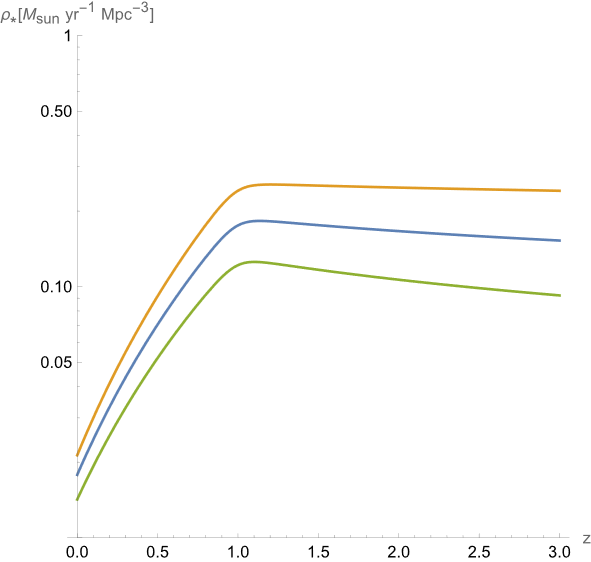
\includegraphics[width=0.5\linewidth]{figures/dsnb/CSFH.png}
    \caption{Star formation rates, in different models}
    \label{fig:csfh}
\end{figure}

The $\frac{\mathrm{d}N(E')}{\mathrm{d}E'}$ is:
\[\frac{\mathrm{d}N(E')}{\mathrm{d}E'} = \]

\begin{figure}[!htb]
    \centering
    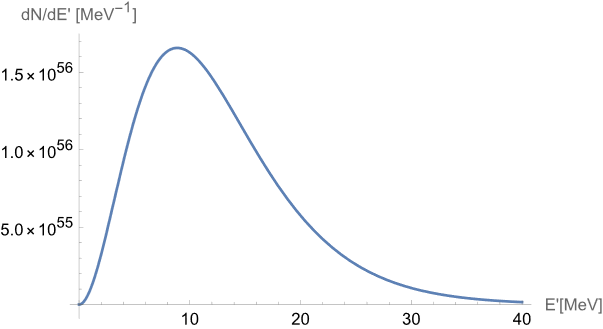
\includegraphics[width=0.5\linewidth]{figures/dsnb/number-emitted.png}
    \caption{Neutrino numbers emitted by one single core collapse supernova}
    \label{fig:number-emitted}
\end{figure}

And the relation between $t$ and $z$ is:
\[\left|\frac{\mathrm{d}t}{\mathrm{d}z}\right| = \]

Finally, the DSNB flux is calculated as figure \ref{fig:dsnb-flux}

\begin{figure}[!htb]
    \centering
    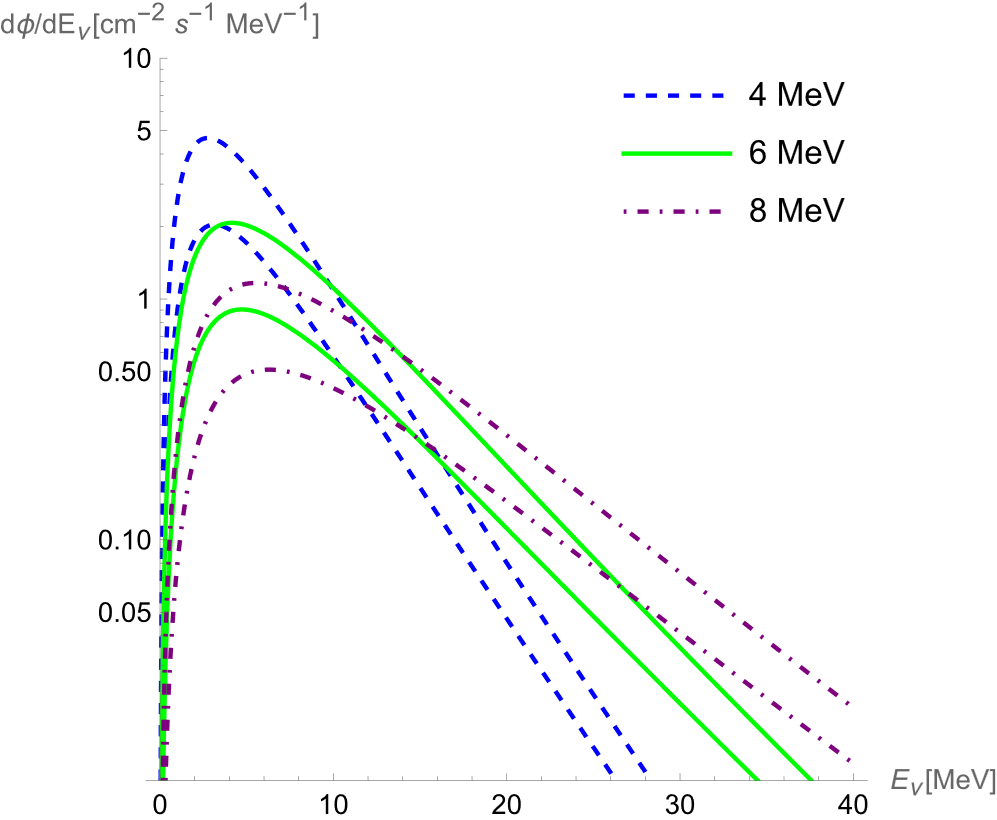
\includegraphics[width=0.5\linewidth]{figures/dsnb/dsnb-flux.png}
    \caption{Calculated DSNB flux. Energies labeled are neutrino temperature after mixing.}
    \label{fig:dsnb-flux}
\end{figure}

\subsection{DSNB interactions and expected event rate}
The neutrino interaction cross section in the detector is calculated:
\[\]

Then the positron spectrum is calculated by:
\[\]

So, we get the DSNB-induced positron spectrum in figure \ref{fig:dsnb-rate}

\begin{figure}[!htb]
    \centering
    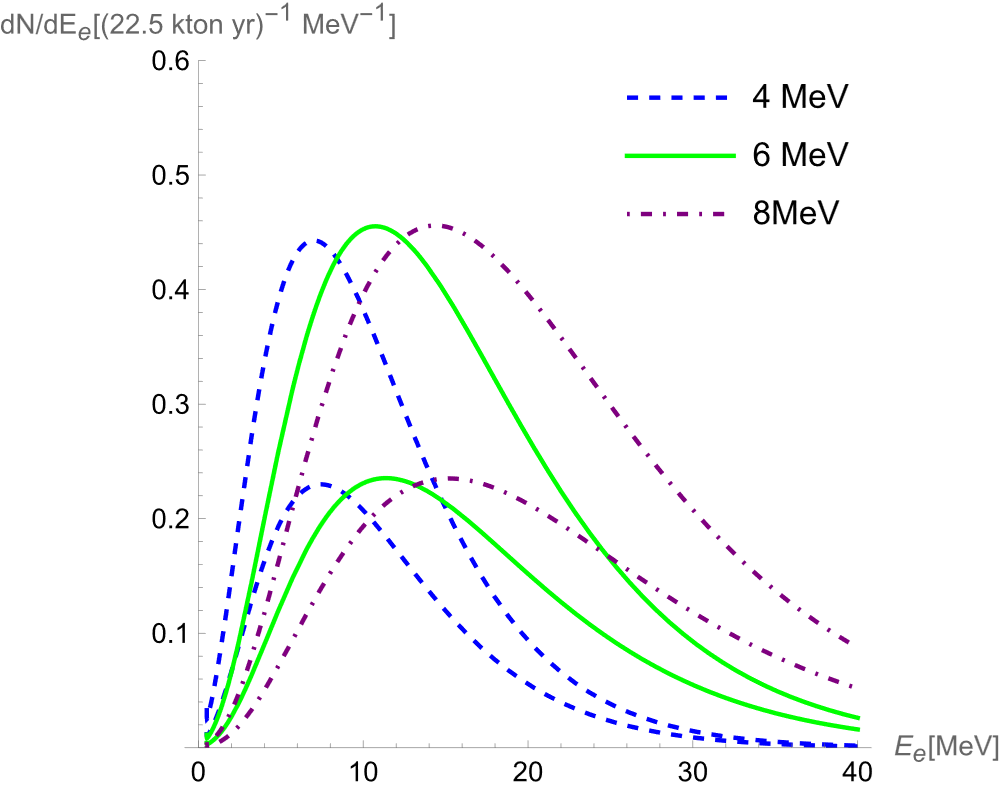
\includegraphics[width=0.5\linewidth]{figures/dsnb/dsnb-rate.png}
    \caption{DSNB rate, with the exposure \SI{22.5}{\kilo\tonne year}}
    \label{fig:dsnb-rate}
\end{figure}

The applied IBD rate induced by DSNB is $2.2 \pm 0.7$, given the neutrino temperature $\SI{6}{\MeV}$ and exposure $\SI{20}{\kilo\tonne year}$

\newpage
\section{Simulation and Event Reconstruction}
\subsection{DSNB and background simulation}
\subsection{vertex reconstruction}

A reconstruction method developed for JNE is applied in this study \cite{luo_reconstruction_2023}. The likelihood function $f(n_i^{obs}, t_{ij}|\vec{\theta})$ shows the probability of observed PE numbers in the i-th PMT $n_i^{obs}$ and their time distributions $t_{ij}$, given vertex $\vec{\theta}$, including the reconstructed energy $E$, position $\{x, y, z\}$, event time $t_{event}$ and direction $\vec{d}_{fit}$.
\begin{equation}
    f(n_i^{obs}, t_{ij} | \vec{\theta})=\prod_i^{N_{PMT}} P_i^C \prod_j^{n_i^{obs}} P_{ij}^T
    \label{equ:likelihood}
\end{equation}

, where

\begin{equation}
    P_i^C = f_{\mathrm{Poisson}}(n_i^{obs}; n_i^{exp})
    \label{equ:likelihood-count}
\end{equation}
\begin{equation}
    P_{ij}^T = \sum{\frac{n_i^{type}}{n_i^{exp}} f^{type} (t_{ij}^{res})}
    \label{equ:likelihood-time}
\end{equation}

The PE number is estimated as: $n_i^{exp} (\vec{\theta}) = \sum{n_i^{type}} (\vec{\theta})$. The time residual is calculated as: $t_{ij}^{res} = t_{ij} - t_{event} - TOF(\vec{\theta}) - t_{shift}$. And its distributions $f^{type}(t)$ are calibrated from simulation.

\subsection{CPE and SPE reconstruction}

\subsubsection{闪烁光 / 切伦科夫光重建方法}

本部分我们将利用模型不依赖的光子时间分布拟合，重建事例的闪烁光 PE 数和切伦科夫光 PE 数

在拟合开始前，我们先计算每个 PE 的光子时间

\begin{equation}
    t_{photon}^C = t_{PE} - \sum_{m} TOF_{m}^{C} - t_{event} - t_{transit}
\end{equation}
  
\begin{equation}
    t_{photon}^S = t_{PE} - \sum_{m} TOF_{m}^{S} - t_{event} - t_{transit}
\end{equation}

其中 $\sum_{m} TOF_{m}$ 表示光子在所有介质中的总飞行时间，三层介质依次为液体闪烁体、亚克力、矿油，光子在介质中的飞行速度与其波长有关，而闪烁光与切伦科夫光的波长组成不同，我们据此应用不同的等效群速度 $v_{m}^{S, eff}, v_{m}^{C, eff}$，分别计算同一个 PE 是闪烁光和切伦科夫光时的飞行时间

$t_{event}$ 表示事例开始的时间，$t_{transit}$ 表示渡越时间，在顶点重建中，它们作为一个整体被重建 $t_0 = t_{event} + t_{transit}$。每个 PE 真实的 $t_{transit}$ 不同，而一个事例中的所有 PE 共用一个 $t_0$，因此根据重建顶点信息计算的 $t_{photon}$ 是经过 TTS 展宽后的光子时间，对于本身光子时间散布较小的直接切伦科夫光，TTS 展宽的效应尤其明显

根据 PE 的光子时间，进行扩展非分箱最大似然拟合：

\begin{equation}
    \mathcal{L} = e^{- \sum_k N_k} \prod_{i=1}^{N_{obs}} \left( \sum_k N_k f_k \right)
\end{equation}

其中 $k$ 表示 PE 的种类，包括直入射闪烁光、非直入射闪烁光、直入射切伦科夫光、非直入射切伦科夫光、暗噪声共 5 种；$N_k$ 表示每种类型的光的 PE 数，是待拟合参数；$f_k$ 是展宽后的光子时间分布（光强曲线）

对于直入射切伦科夫光

\begin{equation}
    f^{CD} (t_{photon}^C) = \delta(t_{photon}^C) \otimes \mathrm{Gauss} (0, \sigma_{tt})
\end{equation}

对于闪烁光、非直入射切伦科夫光

\begin{equation}
    f^k (t_{photon}) = \frac{\tau_r^k + \tau_d^k}{{\tau_d^k}^2} (1 - e^{-t_{photon} / \tau_r^k} e^{-t_{photon} / \tau_d^k} \otimes \mathrm{Gauss} (0, \sigma_{tt}))
\end{equation}

在模拟研究中，PMT 的 TTS 设定为 FWHM \SI{1}{\nano \second}，所以高斯标准差 $\sigma_{tt} = \SI{0.424}{\nano\second}$，其他参数设置见表 \ref{tab:light-param}

\begin{table}[!htb]
    \centering
    \caption{直入射闪烁光（SD）、非直入射闪烁光（SI）、直入射切伦科夫光（CD）、非直入射切伦科夫光（CI）光强曲线参数}
    \begin{tabular}{ccccc}
        \hline
        & CD & CI & SD & SI \\
        \hline
        $\tau_r [\si{\nano\second}]$ & - & 0.211 & 0.5 & 6.20 \\
        $\tau_d [\si{\nano\second}]$ & - & 14.1 & 10 & 19.7 \\
        $\sigma_{tt} [\si{\nano\second}]$ & 0.424 & 0.424 & 0.424 & 0.424 \\
        \hline
    \end{tabular}
    \label{tab:light-param}
\end{table}

图 \ref{fig:e-sd} 展示了直入射闪烁光时间分布，图 \ref{fig:e-cd} 展示了直入射切伦科夫光时间分布。可以看到，\SI{3}{\MeV} 电子直入射闪烁光的展宽光子时间分布成分主要是闪烁光发光时延，由液闪介质决定；直入射切伦科夫光的展宽光子时间分布成分主要是 PMT 渡越时间，由 PMT 结构决定 

\begin{figure}[!htb]
    \centering
    \subfigure[带电粒子沉积能量时间分布]{
        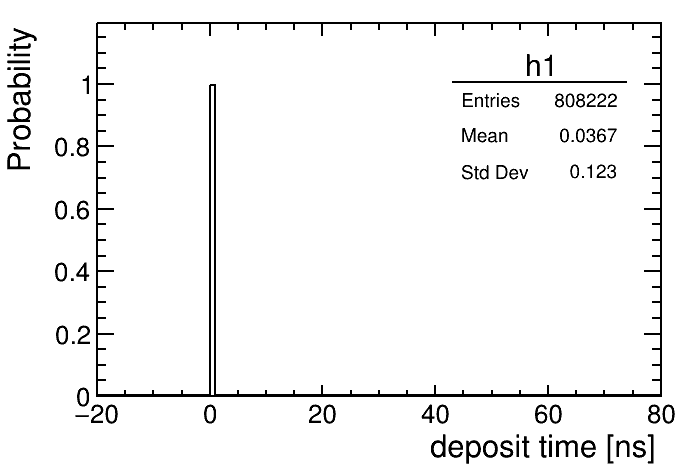
\includegraphics[width=0.45\linewidth]{figures/sim-recon/pe-beta/s-dep.png}
    }
    \subfigure[闪烁光发光时延]{
        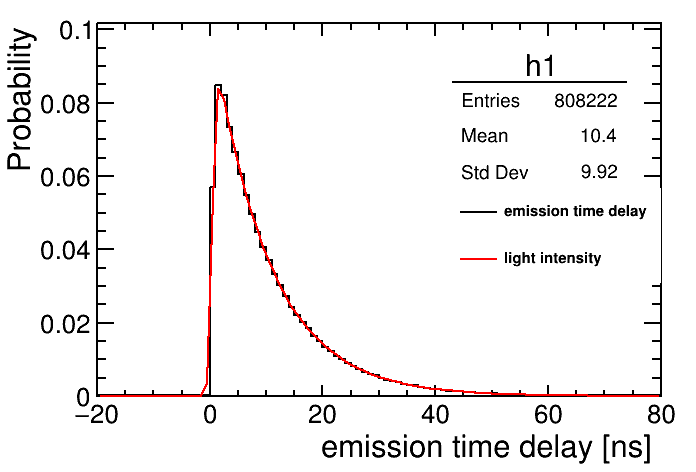
\includegraphics[width=0.45\linewidth]{figures/sim-recon/pe-beta/s-tdelay.png} 
    }
    \subfigure[光子时间]{
        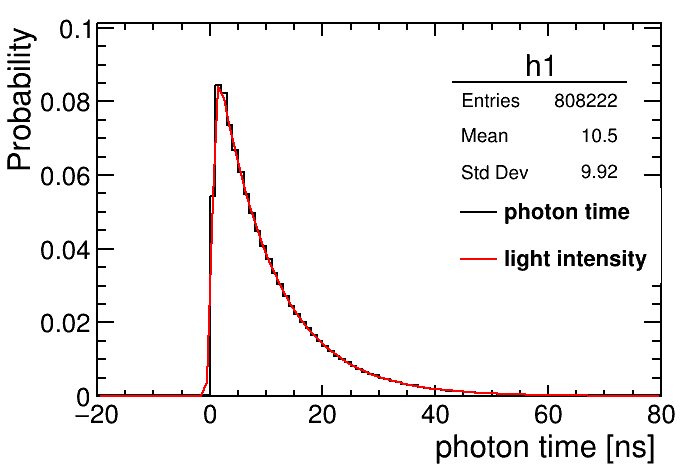
\includegraphics[width=0.45\linewidth]{figures/sim-recon/pe-beta/s-pho.png}
    }
    \subfigure[TTS 展宽的光子时间]{
        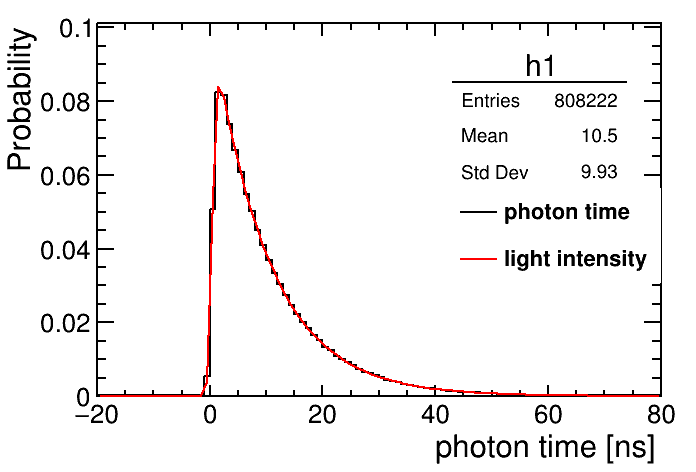
\includegraphics[width=0.45\linewidth]{figures/sim-recon/pe-beta/s-pho-smear.png}
    }
    \caption{模拟的 \SI{3}{\MeV} 电子直入射闪烁光 PE 时间分布真值。模拟的闪烁光光强曲线设置 $\tau_r = \SI{0.5}{\nano\second}$, $\tau_d = \SI{10}{\nano\second}$，PMT 渡越时间 $FWHM = \SI{1}{\nano\second}$。红线表示拟合用的直入射闪烁光 PE 时间分布，参数见表 \ref{tab:light-param}}
    \label{fig:e-sd}
\end{figure}

\begin{figure}[!htb]
    \centering
    \subfigure[带电粒子沉积能量时间分布]{
        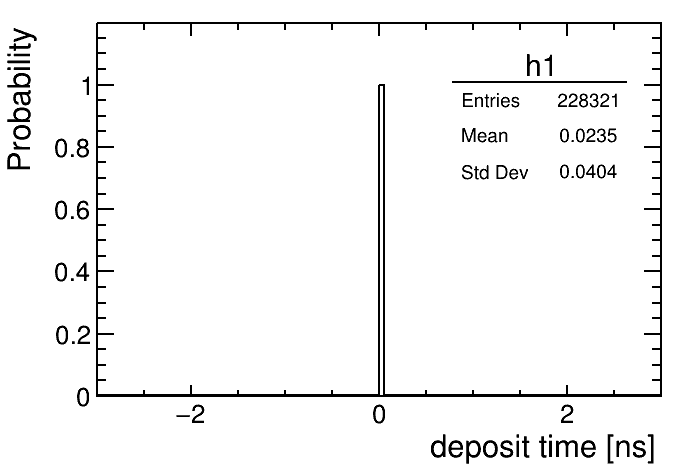
\includegraphics[width=0.45\linewidth]{figures/sim-recon/pe-beta/c-dep.png}
    }
    \subfigure[闪烁光发光时延]{
        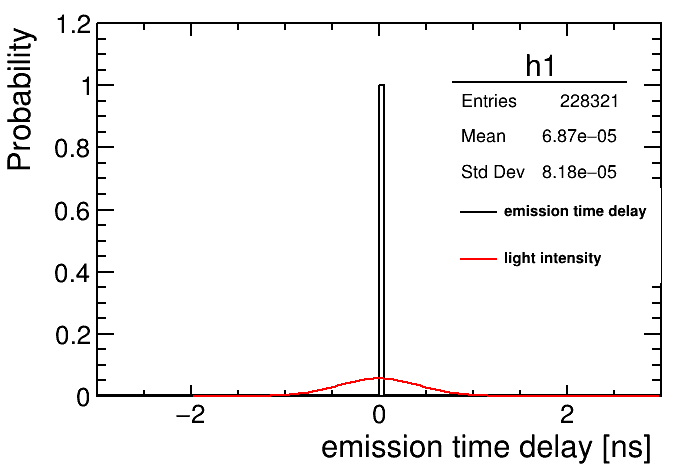
\includegraphics[width=0.45\linewidth]{figures/sim-recon/pe-beta/c-tdelay.png} 
    }
    \subfigure[光子时间]{
        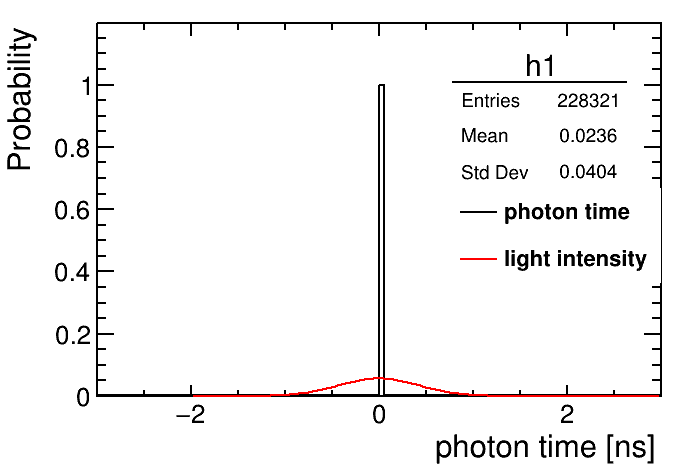
\includegraphics[width=0.45\linewidth]{figures/sim-recon/pe-beta/c-pho.png}
    }
    \subfigure[TTS 展宽的光子时间]{
        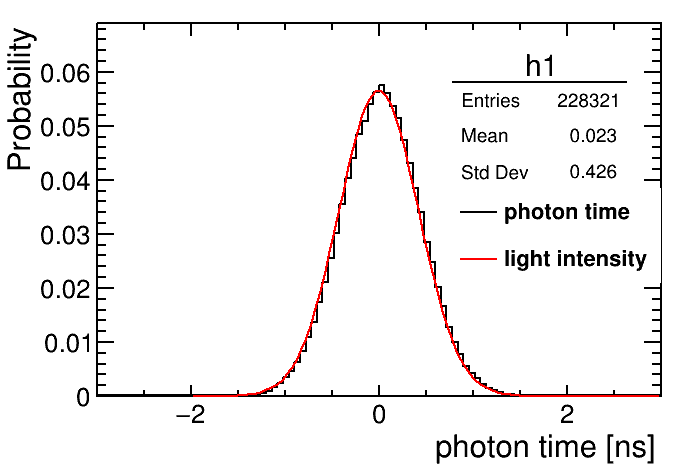
\includegraphics[width=0.45\linewidth]{figures/sim-recon/pe-beta/c-pho-smear.png}
    }
    \caption{模拟的 \SI{3}{\MeV} 电子直入射切伦科夫光 PE 时间分布真值。模拟的设定的PMT 渡越时间 $FWHM = \SI{1}{\nano\second}$。红线表示拟合用的直入射切伦科夫光 PE 时间分布，参数见表 \ref{tab:light-param}}
    \label{fig:e-cd}
\end{figure}

\subsubsection{电子和中子重建效果}    
\subsubsection{中子重建效果不佳的原因}


\subsection{CPE and SPE reconstruction}
% 本研究采用的

% CPE 和 SPE 的重建，主要由 PE 的时间残差 $t^{res}$ 决定，同时也受到电子模型预测的影响，总体上是模型无关的。也就是说，该方法重建的闪烁光 / 切伦科夫光 PE 比例可以反应不同粒子切伦科夫光光产额的不同。

% 具体计算方法：对于 PMT i 上的 PE j，先基于时间；再基于电子模型，计算 PMT i 上各类型（闪烁光 / 切伦科夫光 * 直入射 / 非直入射 + 暗噪声）的 PE 期望数 $\nu_i^{type} (\vec{\theta})$

在本部分，我们讨论如何确定某个特定 PMT 上的某个特定 PE 是闪烁光 / 切伦科夫光 PE，我们计算它是闪烁光 / 切伦科夫光的概率 $P_c, P_s$。我们已知 PE 的 hit 时间 $t^{hit}$

在计算前，我们已有拟合结果：
\begin{equation}
    \vec{\theta} = (E, t_0, \vec{x}, \vec{d})
\end{equation}

由此可以得到 PMT 上的闪烁光 / 切伦科夫光 PE 数预期：
\begin{equation}
    \left\{
    \begin{aligned}
        & n_c = n_c^{pred}(\vec{\theta}, e^- model) \\
        & n_s = n_s^{pred}(\vec{\theta}, e^- model)
    \end{aligned}
    \right.
\end{equation}

$n_c, n_s$ 在顶点确定之后，就能由电子模型计算出唯一值

另外我们可以计算 PE 的光子时间，以及它们满足的概率分布：
\begin{equation}
    t^{photon} = t^{hit} - t_0 - TOF(\vec{\theta}) - TT
\end{equation}

\begin{equation}
    \left\{
    \begin{aligned}
        & f_c = P(t = t^{photon} | Cherenkov, LiCl scintillator) \\
        & f_s = P(t = t^{photon} | Scintillation, LiCl scintillator)
    \end{aligned}
    \right.
\end{equation}

概率分布由液闪性质决定，且闪烁光与切伦科夫光的概率分布不同

在当前的算法中，一个 PE 是切伦科夫 PE 的概率计算为：

\begin{equation}
    \begin{aligned}
        P_c & = \frac{n_c f_c}{n_c f_c + n_s f_s} \\
        N_c & = \sum_{All PE} P_c
    \end{aligned}
    \label{equ:nc-recon}
\end{equation}

可以观察到

\begin{equation}
    \begin{aligned}
        P_c & = \frac{n_c f_c}{n_c f_c + n_s f_s} \\
        & = \frac{\frac{n_c}{n_c + n_s} f_c}{\frac{n_c}{n_c + n_s} f_c + \frac{n_c}{n_c + n_s} f_s} \\
        & = \frac{P(c) P(t|c)}{P(c) P(t|c) + P(s) P(t|s)} \\
    \end{aligned}
\end{equation}



可见，所求为已知 PE 光子时间的后验概率 $P(c|t)$，而这里的先验概率
\begin{equation}
    P(c) = \frac{n_c}{n_c + n_s}
\end{equation}

是电子模型下，没有时间信息时，特定 PMT 中一个 PE 是切伦科夫 PE 的概率。在我们不知道粒子种类时，没有这个先验概率，所以这里确实应该修改。

对于不知种类的粒子事例，一个 PE 是切伦科夫 PE 的概率为：
\begin{equation}
    P_c = \frac{f_c}{f_c + f_s}
\end{equation}

\newpage
\section{Atmospheric-neutrino Background}
Background:
\begin{itemize}
    \item cosmic ray muons
    \item reactor neutrinos
    \item atmospheric neutrinos
\end{itemize}

Given the features of Jinping 500-ton neutrino detector, the former two can be ignored, and the atmospheric neutrinos are discussed.

\subsection{Atmos neutrinos flux and event rate estimation}
\label{sec:atmos-rate}
% Honda, Kajita, T., Kasahara, K., & Midorikawa, S. (2011). Improvement of low energy atmospheric neutrino flux calculation using the JAM nuclear interaction model. Physical Review. D, Particles and Fields, 83(12). 

% Zhou, & Beacom, J. F. (2024). First Detailed Calculation of Atmospheric Neutrino Foregrounds to the Diffuse Supernova Neutrino Background in Super-Kamiokande.


The flux and xsec are shown in figure \ref{fig:atmos-e} and figure \ref{fig:atmos-mu}

\begin{figure}[!htb]
    \centering
    \subfigure[]{
        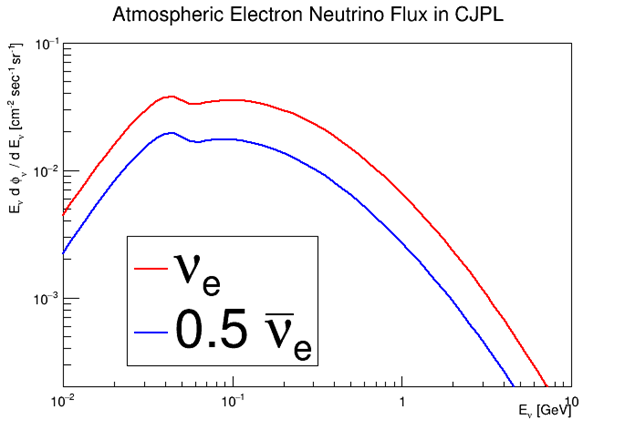
\includegraphics[width=0.45\linewidth]{figures/background/atmos-flux-e.png}
    }
    \subfigure[]{
        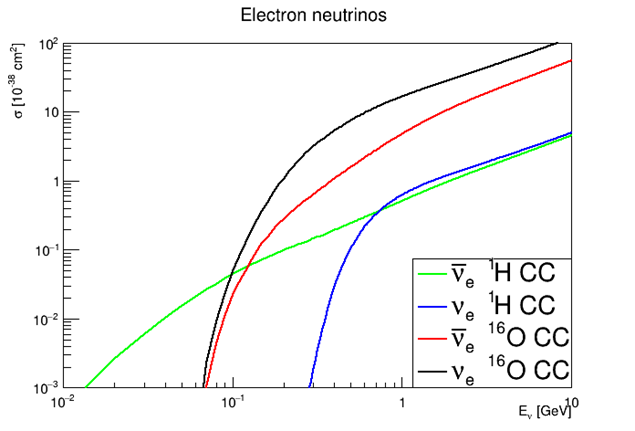
\includegraphics[width=0.45\linewidth]{figures/background/atmos-xsec-e.png} 
    }
    \caption{$\nu_e$ and $\bar{\nu}_e$ fluxes and cross sections with \ce{O} and \ce{H}}
    \label{fig:atmos-e}
\end{figure}

\begin{figure}[!htb]
    \centering
    \subfigure[]{
        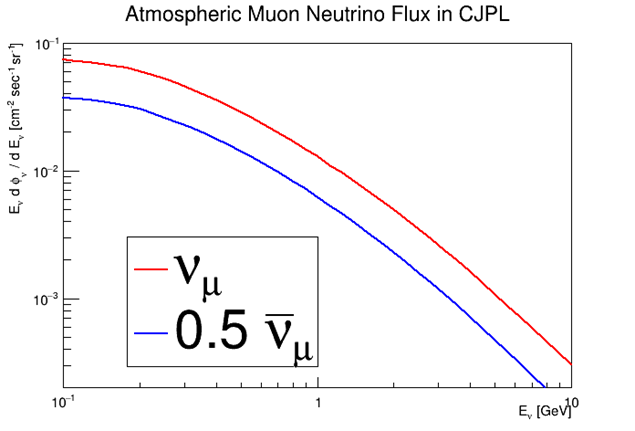
\includegraphics[width=0.45\linewidth]{figures/background/atmos-flux-mu.png}
    }
    \subfigure[]{
        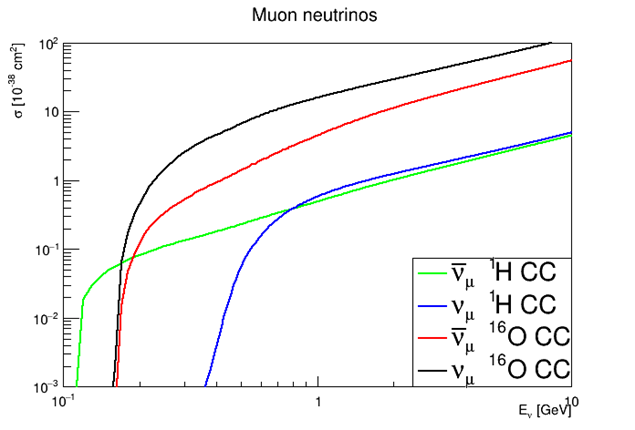
\includegraphics[width=0.45\linewidth]{figures/background/atmos-xsec-mu.png} 
    }
    \caption{$\nu_{\mu}$ and $\bar{\nu}_{\mu}$ fluxes and cross sections with \ce{O} and \ce{H}}
    \label{fig:atmos-mu}
\end{figure}

The integrated event rates are shown in table \ref{tab:atmos-rate}

\begin{table}[!htb]
    \caption{Atmospheric neutrino event rates, where the exposure is \SI{20}{\kilo \tonne \cdot year}}
    \begin{tabular}{rrrrr}
        \hline
         & $\nu_e$ & $\bar{\nu}_e$ & $\nu_{\mu}$ & $\bar{\nu}_{\mu}$ \\
        \hline
        \ce{^{1}H} & 0.52 & 0.21 & 1.0 & 0.61 \\
        \ce{^{2}H} & $2.6 \times 10^{-5}$ & $1.4 \times 10^{-5}$ & $9.2 \times 10^{-5}$ & $4.6 \times 10^{-5}$ \\
        \ce{^{6}Li} & $1.3 \times 10^{-2}$ & $0.49 \times 10^{-2}$ & $3.8 \times 10^{-2}$ & $1.5 \times 10^{-2}$ \\
        \ce{^{7}Li} & 0.18 & 0.0070 & 0.55 & 0.21 \\
        \ce{^{16}O} & 1.1 & 0.40 & 2.9 & 1.1 \\
        \ce{^{18}O} & $2.5 \times 10^{-3}$ & $0.91 \times 10^{-3}$ & $6.8 \times 10^{-3}$ & $2.4 \times 10^{-3}$ \\
        \ce{^{35}Cl} & 0.97 & 0.35 & 2.5 & 0.94 \\
        \ce{^{37}Cl} & 0.33 & 0.11 & 0.84 & 0.27 \\
        Total & 3.12 & 1.16 & 7.87 & 3.19 \\
        \hline
    \end{tabular}
    \label{tab:atmos-rate}
\end{table}

\subsection{Final-state classification}
在 \ref{sec:atmos-rate} 中，我们计算了不同种类大气中微子的通量，以及它们和探测器内各种核素反应的事例率。现在我们将不同的末态分开统计

反应可以分为 NC、CC 两类。NC 过程末态为中微子、核子和末态核，CC 过程末态包括带电轻子、核子和末态核

末态核子数量不同，反应原理不同，可能导致末态事例特征的变化，如 $\ce{^{16}O} + \bar{\nu}_e$ NC 末态，中子数量为 1 个或多个，中子能谱有较大不同；此外，末态核子数量不同，导致末态反冲核也不同，不同的反冲核具有不同的行为，如 $\ce{^{6}Li} + \bar{\nu}_e$ NC 末态，当末态质子数量为 1 个时，产生低寿命 $\ce{^{5}He}$，快速衰变，而当末态质子数量为多个时，产生其他较稳定的核素。因此，我们有必要核子数量不同的末态分开讨论。

根据末态中子的数量 $(0, 1, \ge 2)$ 和末态质子的数量 $(0, 1, \ge 2)$，我们将 NC 末态分为 $3 \times 3 - 1 = 8$ 类。带介子的末态，或中微子与核外电子散射的末态，数量较少，单独分为一类，一共 9 类。

\begin{table}[!htb]
    \centering
    \caption{大气中微子 NC 末态}
    \begin{tabular}{c|ccc}
        \diagbox{中子数}{质子数} & $0$ & $1$ & $\ge 2$ \\
        \hline
        $0$ & - & $p + \nu + N$ & $p's + \nu + N$ \\
        $1$ & $n + \nu + N$ & $n + p + \nu + N$ & $n + p's + \nu + N$ \\
        $\ge 2$ & $n's + \nu + N$ & $n's + p + \nu + N$ & $n's + p's + \nu + N$ \\
    \end{tabular}
\end{table}

对于 NC 末态，我们也进行同样的分类，只是对于 $\nu_e, \nu_{\mu}$，末态无中子；对于 $\bar{\nu}_e, \bar{\nu}_{\mu}$，末态无质子。故末态一共分为 7 类。

统计通过 GENIE 模拟的 $N + \nu$ 末态，统计每个末态占模拟总数的比例，形成如下表格（表中只展示 $\bar{\nu}_e$ 末态）：

\begin{table}[!htb]
    \centering
    \caption{$\bar{\nu}_e$ 与不同核素反应 NC 末态}
    \begin{tabular}{c|ccccccccc}
    \hline
        ~ & NC & \makecell{$n+$ \\ $\nu+N$} & \makecell{$n's+$ \\ $\nu+N$} & \makecell{$p+$ \\ $\nu+N$} & \makecell{$p's+$ \\ $\nu+N$} & \makecell{$n+p+$ \\ $\nu+N$} & \makecell{$n's+p+$ \\ $\nu+N$} & \makecell{$n+p's+$ \\ $\nu+N$} & \makecell{$n's+p's+$ \\ $\nu+N$}  \\
        \hline
        H-1 & 83.0\% & ~ & ~ & 82.9\% & ~ & ~ & ~ & ~ &   \\
        H-2 & 91.7\% & 25.5\% & ~ & ~ & ~ & 66.0\% & ~ & ~ &   \\
        Li-6 & 94.6\% & 28.2\% & 2.9\% & 38.9\% & 3.9\% & 13.6\% & 2.0\% & 2.4\% & 2.2\%  \\
        Li-7 & 95.0\% & 33.3\% & 3.5\% & 32.2\% & 2.1\% & 10.1\% & 5.4\% & 3.3\% & 4.6\%  \\
        C-12 & 95.2\% & 27.5\% & 2.5\% & 37.1\% & 3.2\% & 8.2\% & 3.7\% & 4.1\% & 8.0\%  \\
        C-13 & 95.7\% & 31.5\% & 2.9\% & 35.5\% & 2.4\% & 7.6\% & 4.3\% & 3.3\% & 7.4\%  \\
        O-16 & 96.5\% & 30.2\% & 3.5\% & 32.5\% & 3.6\% & 9.0\% & 4.3\% & 4.4\% & 8.2\%  \\
        O-18 & 96.7\% & 33.1\% & 4.7\% & 28.0\% & 3.0\% & 8.9\% & 5.6\% & 3.9\% & 8.7\%  \\
        Cl-35 & 97.2\% & 23.9\% & 4.8\% & 29.4\% & 5.5\% & 9.9\% & 6.0\% & 6.0\% & 11.2\%  \\
        Cl-37 & 97.3\% & 25.1\% & 5.4\% & 27.9\% & 5.1\% & 10.1\% & 6.6\% & 5.5\% & 11.2\%  \\
    \end{tabular}
\end{table}

\begin{table}[!htb]
    \centering
    \caption{$\bar{\nu}_e$ 与不同核素反应 CC 末态}
    \begin{tabular}{c|ccccccc}
        ~ & CC & \makecell{$n+$ \\ $e^-+N$} & \makecell{$n's+$ \\ $e^-+N$} & \makecell{$n+p+$ \\ $e^-+N$} & \makecell{$n's+p+$ \\ $e^-+N$} & \makecell{$n+p's+$ \\ $e^-+N$} & \makecell{$n's+p's+$ \\ $e^-+N$} \\
        \hline
        H-1 & 17.0\% & 17.0\% & ~ & ~ & ~ & ~ &   \\ 
        H-2 & 8.3\% & ~ & 8.2\% & ~ & ~ & ~ &   \\ 
        Li-6 & 5.4\% & 3.7\% & 0.8\% & 0.5\% & 0.2\% & 0.0\% & 0.1\%  \\ 
        Li-7 & 5.0\% & 3.4\% & 0.7\% & 0.2\% & 0.4\% & 0.0\% & 0.1\%  \\ 
        C-12 & 4.8\% & 2.7\% & 0.6\% & 0.4\% & 0.4\% & 0.1\% & 0.4\%  \\ 
        C-13 & 4.3\% & 2.5\% & 0.6\% & 0.3\% & 0.4\% & 0.1\% & 0.3\%  \\ 
        O-16 & 3.5\% & 2.0\% & 0.5\% & 0.2\% & 0.3\% & 0.1\% & 0.2\%  \\ 
        O-18 & 3.3\% & 1.9\% & 0.4\% & 0.2\% & 0.3\% & 0.0\% & 0.2\%  \\ 
        Cl-35 & 2.8\% & 1.4\% & 0.4\% & 0.2\% & 0.3\% & 0.1\% & 0.3\%  \\ 
        Cl-37 & 2.7\% & 1.3\% & 0.4\% & 0.2\% & 0.3\% & 0.1\% & 0.2\%  \\ 
    \end{tabular}
\end{table}

现在我们将每种核素与 $\bar{\nu}_e$ 反应的末态比例绘制成一张折线图，并将所有核素的折线图汇总到一张图中，从而直观感受它们的异同。图中“比例偏差”表示此种核素相对各核素均值的偏差

\begin{figure}[!htb]
    \centering
    \subfigure[NC 各末态比例]{
        \includegraphics[width=0.45\linewidth]{../../dsnb/data/final_state_plots/nue_nc_ratio.png}
    }
    \subfigure[NC 各末态比例偏差]{
        \includegraphics[width=0.45\linewidth]{../../dsnb/data/final_state_plots/nue_nc_deviation.png} 
    }
    \subfigure[CC 各末态比例]{
        \includegraphics[width=0.45\linewidth]{../../dsnb/data/final_state_plots/nue_cc_ratio.png}
    }
    \subfigure[CC 各末态比例偏差]{
        \includegraphics[width=0.45\linewidth]{../../dsnb/data/final_state_plots/nue_cc_deviation.png}
    }
    \caption{$\nu_e$ 与各核素反应末态各成分比例}
\end{figure}

\begin{figure}[!htb]
    \centering
    \subfigure[NC 各末态比例]{
        \includegraphics[width=0.45\linewidth]{../../dsnb/data/final_state_plots/nuebar_nc_ratio.png}
    }
    \subfigure[NC 各末态比例偏差]{
        \includegraphics[width=0.45\linewidth]{../../dsnb/data/final_state_plots/nuebar_nc_deviation.png} 
    }
    \subfigure[CC 各末态比例]{
        \includegraphics[width=0.45\linewidth]{../../dsnb/data/final_state_plots/nuebar_cc_ratio.png}
    }
    \subfigure[CC 各末态比例偏差]{
        \includegraphics[width=0.45\linewidth]{../../dsnb/data/final_state_plots/nuebar_cc_deviation.png}
    }
    \caption{$\bar{\nu}_e$ 与各核素反应末态各成分比例}
\end{figure}

\begin{figure}[!htb]
    \centering
    \subfigure[NC 各末态比例]{
        \includegraphics[width=0.45\linewidth]{../../dsnb/data/final_state_plots/numu_nc_ratio.png}
    }
    \subfigure[NC 各末态比例偏差]{
        \includegraphics[width=0.45\linewidth]{../../dsnb/data/final_state_plots/numu_nc_deviation.png} 
    }
    \subfigure[CC 各末态比例]{
        \includegraphics[width=0.45\linewidth]{../../dsnb/data/final_state_plots/numu_cc_ratio.png}
    }
    \subfigure[CC 各末态比例偏差]{
        \includegraphics[width=0.45\linewidth]{../../dsnb/data/final_state_plots/numu_cc_deviation.png}
    }
    \caption{$\nu_{\mu}$ 与各核素反应末态各成分比例}
\end{figure}

\begin{figure}[!htb]
    \centering
    \subfigure[NC 各末态比例]{
        \includegraphics[width=0.45\linewidth]{../../dsnb/data/final_state_plots/numubar_nc_ratio.png}
    }
    \subfigure[NC 各末态比例偏差]{
        \includegraphics[width=0.45\linewidth]{../../dsnb/data/final_state_plots/numubar_nc_deviation.png} 
    }
    \subfigure[CC 各末态比例]{
        \includegraphics[width=0.45\linewidth]{../../dsnb/data/final_state_plots/numubar_cc_ratio.png}
    }
    \subfigure[CC 各末态比例偏差]{
        \includegraphics[width=0.45\linewidth]{../../dsnb/data/final_state_plots/numubar_cc_deviation.png}
    }
    \caption{$\bar{\nu}_{\mu}$ 与各核素反应末态各成分比例}
\end{figure}
\newpage
\subsection{Final-state composition and simulated rates}
为了便于讨论，我们将所有的大气中微子事例按三个维度分类，三个维度分别为中微子味道及反应流、核素、末态。

分类的层次和每一层次的经典值见下图所示。

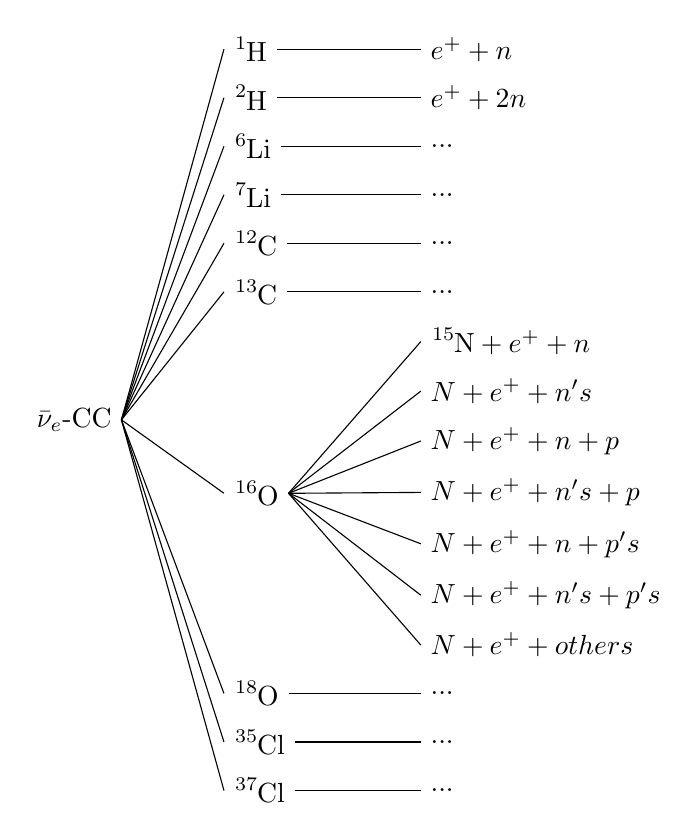
\begin{tikzpicture}[
    grow'=right,
    level distance=2.5cm,
    % sibling distance=1.5cm,
    every tree node/.style={anchor=west},
]
\Tree
[.$\bar{\nu}_e$-CC
    [.\ce{^{1}H} [.$e^++n$ ] ]
    [.\ce{^{2}H} [.$e^++2n$ ] ]
    [.\ce{^{6}Li} [.... ] ]
    [.\ce{^{7}Li} [.... ] ]
    [.\ce{^{12}C} [.... ] ]
    [.\ce{^{13}C} [.... ] ]
    [.\ce{^{16}O}
        [.$\ce{^{15}N}+e^++n$ ]
        [.$N+e^++n's$ ]
        [.$N+e^++n+p$ ]
        [.$N+e^++n's+p$ ]
        [.$N+e^++n+p's$ ]
        [.$N+e^++n's+p's$ ]
        [.$N+e^++others$ ]
    ]
    [.\ce{^{18}O} [.... ] ]
    [.\ce{^{35}Cl} [.... ] ]
    [.\ce{^{37}Cl} [.... ] ]
]
\end{tikzpicture}

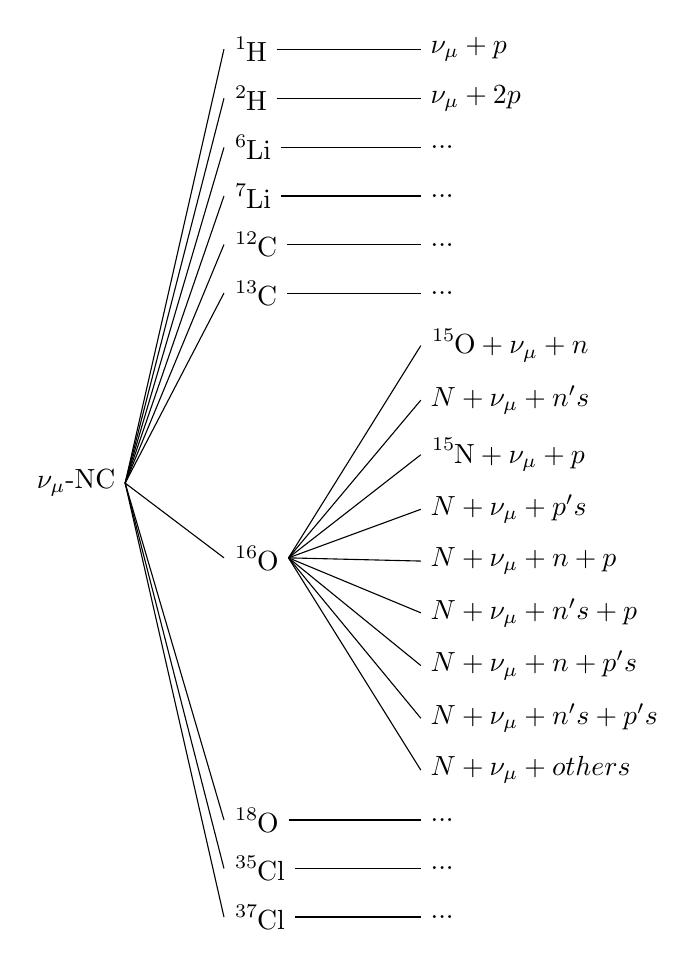
\begin{tikzpicture}[
    grow'=right,
    level distance=2.5cm,
    % sibling distance=1.5cm,
    every tree node/.style={anchor=west},
]
\Tree
[.$\nu_{\mu}$-NC
    [.\ce{^{1}H} [.$\nu_{\mu}+p$ ] ]
    [.\ce{^{2}H} [.$\nu_{\mu}+2p$ ] ]
    [.\ce{^{6}Li} [.... ] ]
    [.\ce{^{7}Li} [.... ] ]
    [.\ce{^{12}C} [.... ] ]
    [.\ce{^{13}C} [.... ] ] 
    [.\ce{^{16}O}
        [.$\ce{^{15}O}+\nu_{\mu}+n$ ]
        [.$N+\nu_{\mu}+n's$ ]
        [.$\ce{^{15}N}+\nu_{\mu}+p$ ]
        [.$N+\nu_{\mu}+p's$ ]
        [.$N+\nu_{\mu}+n+p$ ]
        [.$N+\nu_{\mu}+n's+p$ ]
        [.$N+\nu_{\mu}+n+p's$ ]
        [.$N+\nu_{\mu}+n's+p's$ ]
        [.$N+\nu_{\mu}+others$ ]
    ]
    [.\ce{^{18}O} [.... ] ]
    [.\ce{^{35}Cl} [.... ] ]
    [.\ce{^{37}Cl} [.... ] ]
]
\end{tikzpicture}

下表将展示每类大气中微子事例在 \SI{20}{\kilo\tonne year} 曝光量下的实际事例率和模拟的事例数

\newpage
\begin{table}[!htb]
    \centering
    \caption{$\nu_e$ 各类事例实际事例率和模拟事例数}
    \resizebox{\textwidth}{!}{%
    \begin{tabular}{c|cccccccccc}
        \hline
         & \ce{^{1}H} & \ce{^{2}H} & \ce{^{6}Li} & \ce{^{7}Li} & \ce{^{12}C} & \ce{^{13}C} & \ce{^{16}O} & \ce{^{18}O} & \ce{^{35}Cl} & \ce{^{37}Cl} \\
        \thickhline
        \textbf{NC} & \makecell{\boldmath$0.52$ \\ \boldmath$9989$} & \makecell{\boldmath$2.4\times 10^{-5}$ \\ \boldmath$9339$} & \makecell{\boldmath$1.3\times 10^{-2}$ \\ \boldmath$9638$} & \makecell{\boldmath$0.17$ \\ \boldmath$9607$} & \makecell{\boldmath$0$ \\ \boldmath$9632$} & \makecell{\boldmath$0$ \\ \boldmath$9676$} & \makecell{\boldmath$1.1$ \\ \boldmath$9699$} & \makecell{\boldmath$2.4\times 10^{-3}$ \\ \boldmath$9635$} & \makecell{\boldmath$0.95$ \\ \boldmath$9764$} & \makecell{\boldmath$0.32$ \\ \boldmath$9752$} \\
        \hline
        $N+\nu_e+n$ &  & \makecell{$7.6\times 10^{-6}$ \\ $2935$} & \makecell{$4.4\times 10^{-3}$ \\ $3372$} & \makecell{$6.9\times 10^{-2}$ \\ $3826$} & \makecell{$0$ \\ $3188$} & \makecell{$0$ \\ $3564$} & \makecell{$0.37$ \\ $3379$} & \makecell{$9.2\times 10^{-4}$ \\ $3674$} & \makecell{$0.25$ \\ $2527$} & \makecell{$8.9\times 10^{-2}$ \\ $2711$} \\
        \hline
        $N+\nu_e+n's$ &  &  & \makecell{$4.2\times 10^{-4}$ \\ $325$} & \makecell{$7.2\times 10^{-3}$ \\ $402$} & \makecell{$0$ \\ $329$} & \makecell{$0$ \\ $363$} & \makecell{$4.5\times 10^{-2}$ \\ $406$} & \makecell{$1.3\times 10^{-4}$ \\ $511$} & \makecell{$5.6\times 10^{-2}$ \\ $575$} & \makecell{$2.1\times 10^{-2}$ \\ $626$} \\
        \hline
        $N+\nu_e+p$ & \makecell{$0.52$ \\ $9982$} &  & \makecell{$4.7\times 10^{-3}$ \\ $3606$} & \makecell{$5.2\times 10^{-2}$ \\ $2877$} & \makecell{$0$ \\ $3346$} & \makecell{$0$ \\ $3144$} & \makecell{$0.32$ \\ $2870$} & \makecell{$6.1\times 10^{-4}$ \\ $2443$} & \makecell{$0.25$ \\ $2585$} & \makecell{$8.0\times 10^{-2}$ \\ $2439$} \\
        \hline
        $N+\nu_e+p's$ &  &  & \makecell{$4.5\times 10^{-4}$ \\ $346$} & \makecell{$3.4\times 10^{-3}$ \\ $189$} & \makecell{$0$ \\ $312$} & \makecell{$0$ \\ $244$} & \makecell{$4.1\times 10^{-2}$ \\ $370$} & \makecell{$6.6\times 10^{-5}$ \\ $263$} & \makecell{$4.8\times 10^{-2}$ \\ $500$} & \makecell{$1.5\times 10^{-2}$ \\ $448$} \\
        \hline
        $N+\nu_e+n+p$ &  & \makecell{$1.7\times 10^{-5}$ \\ $6378$} & \makecell{$1.7\times 10^{-3}$ \\ $1275$} & \makecell{$1.9\times 10^{-2}$ \\ $1032$} & \makecell{$0$ \\ $862$} & \makecell{$0$ \\ $804$} & \makecell{$0.11$ \\ $976$} & \makecell{$2.3\times 10^{-4}$ \\ $914$} & \makecell{$0.10$ \\ $1064$} & \makecell{$3.5\times 10^{-2}$ \\ $1047$} \\
        \hline
        $N+\nu_e+n's+p$ &  &  & \makecell{$3.0\times 10^{-4}$ \\ $227$} & \makecell{$9.5\times 10^{-3}$ \\ $528$} & \makecell{$0$ \\ $359$} & \makecell{$0$ \\ $444$} & \makecell{$4.8\times 10^{-2}$ \\ $432$} & \makecell{$1.5\times 10^{-4}$ \\ $617$} & \makecell{$6.4\times 10^{-2}$ \\ $658$} & \makecell{$2.3\times 10^{-2}$ \\ $696$} \\
        \hline
        $N+\nu_e+n+p's$ &  &  & \makecell{$2.8\times 10^{-4}$ \\ $215$} & \makecell{$5.6\times 10^{-3}$ \\ $311$} & \makecell{$0$ \\ $392$} & \makecell{$0$ \\ $344$} & \makecell{$4.5\times 10^{-2}$ \\ $410$} & \makecell{$9.4\times 10^{-5}$ \\ $377$} & \makecell{$5.9\times 10^{-2}$ \\ $607$} & \makecell{$1.9\times 10^{-2}$ \\ $563$} \\
        \hline
        $N+\nu_e+n's+p's$ &  &  & \makecell{$3.0\times 10^{-4}$ \\ $230$} & \makecell{$7.2\times 10^{-3}$ \\ $401$} & \makecell{$0$ \\ $770$} & \makecell{$0$ \\ $711$} & \makecell{$9.2\times 10^{-2}$ \\ $836$} & \makecell{$2.0\times 10^{-4}$ \\ $817$} & \makecell{$0.12$ \\ $1203$} & \makecell{$3.9\times 10^{-2}$ \\ $1174$} \\
        \hline
        $N+\nu_e+$ others & \makecell{$3.6\times 10^{-4}$ \\ $7$} & \makecell{$6.8\times 10^{-8}$ \\ $26$} & \makecell{$5.5\times 10^{-5}$ \\ $42$} & \makecell{$7.4\times 10^{-4}$ \\ $41$} & \makecell{$0$ \\ $74$} & \makecell{$0$ \\ $58$} & \makecell{$2.2\times 10^{-3}$ \\ $20$} & \makecell{$4.8\times 10^{-6}$ \\ $19$} & \makecell{$4.4\times 10^{-3}$ \\ $45$} & \makecell{$1.6\times 10^{-3}$ \\ $48$} \\
        \thickhline
        \textbf{CC} & \makecell{\boldmath$5.7\times 10^{-4}$ \\ \boldmath$11$} & \makecell{\boldmath$1.7\times 10^{-6}$ \\ \boldmath$661$} & \makecell{\boldmath$4.7\times 10^{-4}$ \\ \boldmath$362$} & \makecell{\boldmath$7.1\times 10^{-3}$ \\ \boldmath$393$} & \makecell{\boldmath$0$ \\ \boldmath$368$} & \makecell{\boldmath$0$ \\ \boldmath$324$} & \makecell{\boldmath$3.3\times 10^{-2}$ \\ \boldmath$301$} & \makecell{\boldmath$9.1\times 10^{-5}$ \\ \boldmath$365$} & \makecell{\boldmath$2.3\times 10^{-2}$ \\ \boldmath$236$} & \makecell{\boldmath$8.2\times 10^{-3}$ \\ \boldmath$248$} \\
        \hline
        $N+e^-+p$ &  &  & \makecell{$2.7\times 10^{-4}$ \\ $208$} & \makecell{$3.9\times 10^{-3}$ \\ $218$} & \makecell{$0$ \\ $170$} & \makecell{$0$ \\ $148$} & \makecell{$1.5\times 10^{-2}$ \\ $139$} & \makecell{$4.5\times 10^{-5}$ \\ $180$} & \makecell{$9.1\times 10^{-3}$ \\ $94$} & \makecell{$3.3\times 10^{-3}$ \\ $99$} \\
        \hline
        $N+e^-+p's$ &  & \makecell{$3.1\times 10^{-7}$ \\ $120$} & \makecell{$8.2\times 10^{-5}$ \\ $63$} & \makecell{$9.9\times 10^{-4}$ \\ $55$} & \makecell{$0$ \\ $51$} & \makecell{$0$ \\ $48$} & \makecell{$4.5\times 10^{-3}$ \\ $41$} & \makecell{$9.0\times 10^{-6}$ \\ $36$} & \makecell{$3.6\times 10^{-3}$ \\ $37$} & \makecell{$7.9\times 10^{-4}$ \\ $24$} \\
        \hline
        $N+e^-+n+p$ &  & \makecell{$1.4\times 10^{-6}$ \\ $530$} & \makecell{$5.6\times 10^{-5}$ \\ $43$} & \makecell{$5.6\times 10^{-4}$ \\ $31$} & \makecell{$0$ \\ $31$} & \makecell{$0$ \\ $27$} & \makecell{$3.7\times 10^{-3}$ \\ $34$} & \makecell{$8.3\times 10^{-6}$ \\ $33$} & \makecell{$1.4\times 10^{-3}$ \\ $14$} & \makecell{$9.6\times 10^{-4}$ \\ $29$} \\
        \hline
        $N+e^-+n's+p$ &  &  & \makecell{$3.9\times 10^{-6}$ \\ $3$} & \makecell{$1.3\times 10^{-4}$ \\ $7$} & \makecell{$0$ \\ $6$} & \makecell{$0$ \\ $9$} & \makecell{$8.8\times 10^{-4}$ \\ $8$} & \makecell{$2.2\times 10^{-6}$ \\ $9$} & \makecell{$2.9\times 10^{-4}$ \\ $3$} & \makecell{$5.3\times 10^{-4}$ \\ $16$} \\
        \hline
        $N+e^-+n+p's$ &  &  & \makecell{$3.1\times 10^{-5}$ \\ $24$} & \makecell{$7.6\times 10^{-4}$ \\ $42$} & \makecell{$0$ \\ $32$} & \makecell{$0$ \\ $38$} & \makecell{$2.5\times 10^{-3}$ \\ $23$} & \makecell{$8.8\times 10^{-6}$ \\ $35$} & \makecell{$2.8\times 10^{-3}$ \\ $29$} & \makecell{$6.6\times 10^{-4}$ \\ $20$} \\
        \hline
        $N+e^-+n's+p's$ &  &  & \makecell{$7.8\times 10^{-6}$ \\ $6$} & \makecell{$4.1\times 10^{-4}$ \\ $23$} & \makecell{$0$ \\ $31$} & \makecell{$0$ \\ $26$} & \makecell{$2.2\times 10^{-3}$ \\ $20$} & \makecell{$8.8\times 10^{-6}$ \\ $35$} & \makecell{$3.4\times 10^{-3}$ \\ $35$} & \makecell{$1.1\times 10^{-3}$ \\ $34$} \\
        \hline
        $N+e^-+$ others & \makecell{$5.7\times 10^{-4}$ \\ $11$} & \makecell{$2.9\times 10^{-8}$ \\ $11$} & \makecell{$1.9\times 10^{-5}$ \\ $15$} & \makecell{$3.1\times 10^{-4}$ \\ $17$} & \makecell{$0$ \\ $47$} & \makecell{$0$ \\ $28$} & \makecell{$4.0\times 10^{-3}$ \\ $36$} & \makecell{$9.2\times 10^{-6}$ \\ $37$} & \makecell{$2.3\times 10^{-3}$ \\ $24$} & \makecell{$8.6\times 10^{-4}$ \\ $26$} \\
        \thickhline
        \textbf{total} & \makecell{\boldmath$0.52$ \\ \boldmath$10000$} & \makecell{\boldmath$2.6\times 10^{-5}$ \\ \boldmath$10000$} & \makecell{\boldmath$1.3\times 10^{-2}$ \\ \boldmath$10000$} & \makecell{\boldmath$0.18$ \\ \boldmath$10000$} & \makecell{\boldmath$0$ \\ \boldmath$10000$} & \makecell{\boldmath$0$ \\ \boldmath$10000$} & \makecell{\boldmath$1.1$ \\ \boldmath$10000$} & \makecell{\boldmath$2.5\times 10^{-3}$ \\ \boldmath$10000$} & \makecell{\boldmath$0.97$ \\ \boldmath$10000$} & \makecell{\boldmath$0.33$ \\ \boldmath$10000$} \\
        \hline
    \end{tabular}}
    \label{tab:atmos-detail-nue}
\end{table}

\newpage
\begin{table}[!htb]
    \centering
    \caption{$\bar{\nu}_e$ 各类事例实际事例率和模拟事例数}
    \resizebox{\textwidth}{!}{%
    \begin{tabular}{c|cccccccccc}
        \hline
         & \ce{^{1}H} & \ce{^{2}H} & \ce{^{6}Li} & \ce{^{7}Li} & \ce{^{12}C} & \ce{^{13}C} & \ce{^{16}O} & \ce{^{18}O} & \ce{^{35}Cl} & \ce{^{37}Cl} \\
        \thickhline
        \textbf{NC} & \makecell{\boldmath$0.17$ \\ \boldmath$8274$} & \makecell{\boldmath$1.3\times 10^{-5}$ \\ \boldmath$9189$} & \makecell{\boldmath$4.6\times 10^{-3}$ \\ \boldmath$9481$} & \makecell{\boldmath$6.7\times 10^{-3}$ \\ \boldmath$9518$} & \makecell{\boldmath$0$ \\ \boldmath$9501$} & \makecell{\boldmath$0$ \\ \boldmath$9592$} & \makecell{\boldmath$0.39$ \\ \boldmath$9661$} & \makecell{\boldmath$8.8\times 10^{-4}$ \\ \boldmath$9662$} & \makecell{\boldmath$0.34$ \\ \boldmath$9719$} & \makecell{\boldmath$0.11$ \\ \boldmath$9730$} \\
        \hline
        $N+\bar{\nu}_e+n$ &  & \makecell{$3.6\times 10^{-6}$ \\ $2561$} & \makecell{$1.4\times 10^{-3}$ \\ $2852$} & \makecell{$2.3\times 10^{-3}$ \\ $3336$} & \makecell{$0$ \\ $2709$} & \makecell{$0$ \\ $3121$} & \makecell{$0.12$ \\ $3009$} & \makecell{$3.0\times 10^{-4}$ \\ $3260$} & \makecell{$8.2\times 10^{-2}$ \\ $2355$} & \makecell{$2.7\times 10^{-2}$ \\ $2473$} \\
        \hline
        $N+\bar{\nu}_e+n's$ &  &  & \makecell{$1.5\times 10^{-4}$ \\ $296$} & \makecell{$2.4\times 10^{-4}$ \\ $345$} & \makecell{$0$ \\ $266$} & \makecell{$0$ \\ $287$} & \makecell{$1.4\times 10^{-2}$ \\ $350$} & \makecell{$4.3\times 10^{-5}$ \\ $476$} & \makecell{$1.8\times 10^{-2}$ \\ $501$} & \makecell{$5.5\times 10^{-3}$ \\ $497$} \\
        \hline
        $N+\bar{\nu}_e+p$ & \makecell{$0.17$ \\ $8252$} &  & \makecell{$1.9\times 10^{-3}$ \\ $3816$} & \makecell{$2.3\times 10^{-3}$ \\ $3265$} & \makecell{$0$ \\ $3661$} & \makecell{$0$ \\ $3499$} & \makecell{$0.13$ \\ $3288$} & \makecell{$2.6\times 10^{-4}$ \\ $2906$} & \makecell{$0.10$ \\ $2925$} & \makecell{$3.1\times 10^{-2}$ \\ $2786$} \\
        \hline
        $N+\bar{\nu}_e+p's$ &  &  & \makecell{$1.9\times 10^{-4}$ \\ $387$} & \makecell{$1.5\times 10^{-4}$ \\ $211$} & \makecell{$0$ \\ $326$} & \makecell{$0$ \\ $238$} & \makecell{$1.4\times 10^{-2}$ \\ $357$} & \makecell{$2.8\times 10^{-5}$ \\ $305$} & \makecell{$1.9\times 10^{-2}$ \\ $556$} & \makecell{$5.6\times 10^{-3}$ \\ $506$} \\
        \hline
        $N+\bar{\nu}_e+n+p$ &  & \makecell{$9.2\times 10^{-6}$ \\ $6588$} & \makecell{$6.8\times 10^{-4}$ \\ $1384$} & \makecell{$6.7\times 10^{-4}$ \\ $961$} & \makecell{$0$ \\ $811$} & \makecell{$0$ \\ $758$} & \makecell{$3.5\times 10^{-2}$ \\ $881$} & \makecell{$7.6\times 10^{-5}$ \\ $834$} & \makecell{$3.4\times 10^{-2}$ \\ $968$} & \makecell{$1.1\times 10^{-2}$ \\ $1013$} \\
        \hline
        $N+\bar{\nu}_e+n's+p$ &  &  & \makecell{$1.0\times 10^{-4}$ \\ $211$} & \makecell{$3.9\times 10^{-4}$ \\ $550$} & \makecell{$0$ \\ $390$} & \makecell{$0$ \\ $451$} & \makecell{$1.8\times 10^{-2}$ \\ $445$} & \makecell{$5.0\times 10^{-5}$ \\ $547$} & \makecell{$2.0\times 10^{-2}$ \\ $574$} & \makecell{$6.9\times 10^{-3}$ \\ $631$} \\
        \hline
        $N+\bar{\nu}_e+n+p's$ &  &  & \makecell{$1.3\times 10^{-4}$ \\ $260$} & \makecell{$2.3\times 10^{-4}$ \\ $330$} & \makecell{$0$ \\ $373$} & \makecell{$0$ \\ $337$} & \makecell{$1.8\times 10^{-2}$ \\ $456$} & \makecell{$3.9\times 10^{-5}$ \\ $427$} & \makecell{$2.1\times 10^{-2}$ \\ $607$} & \makecell{$6.5\times 10^{-3}$ \\ $593$} \\
        \hline
        $N+\bar{\nu}_e+n's+p's$ &  &  & \makecell{$9.9\times 10^{-5}$ \\ $202$} & \makecell{$3.2\times 10^{-4}$ \\ $452$} & \makecell{$0$ \\ $817$} & \makecell{$0$ \\ $799$} & \makecell{$3.2\times 10^{-2}$ \\ $797$} & \makecell{$7.7\times 10^{-5}$ \\ $851$} & \makecell{$4.0\times 10^{-2}$ \\ $1150$} & \makecell{$1.3\times 10^{-2}$ \\ $1164$} \\
        \hline
        $N+\bar{\nu}_e+$ others & \makecell{$4.6\times 10^{-4}$ \\ $22$} & \makecell{$5.6\times 10^{-8}$ \\ $40$} & \makecell{$3.6\times 10^{-5}$ \\ $73$} & \makecell{$4.8\times 10^{-5}$ \\ $68$} & \makecell{$0$ \\ $148$} & \makecell{$0$ \\ $102$} & \makecell{$3.1\times 10^{-3}$ \\ $78$} & \makecell{$5.1\times 10^{-6}$ \\ $56$} & \makecell{$2.9\times 10^{-3}$ \\ $83$} & \makecell{$7.4\times 10^{-4}$ \\ $67$} \\
        \thickhline
        \textbf{CC} & \makecell{\boldmath$3.6\times 10^{-2}$ \\ \boldmath$1726$} & \makecell{\boldmath$1.1\times 10^{-6}$ \\ \boldmath$811$} & \makecell{\boldmath$2.5\times 10^{-4}$ \\ \boldmath$519$} & \makecell{\boldmath$3.4\times 10^{-4}$ \\ \boldmath$482$} & \makecell{\boldmath$0$ \\ \boldmath$499$} & \makecell{\boldmath$0$ \\ \boldmath$408$} & \makecell{\boldmath$1.4\times 10^{-2}$ \\ \boldmath$339$} & \makecell{\boldmath$3.1\times 10^{-5}$ \\ \boldmath$338$} & \makecell{\boldmath$9.8\times 10^{-3}$ \\ \boldmath$281$} & \makecell{\boldmath$3.0\times 10^{-3}$ \\ \boldmath$270$} \\
        \hline
        $N+e^++n$ & \makecell{$3.6\times 10^{-2}$ \\ $1726$} &  & \makecell{$1.8\times 10^{-4}$ \\ $371$} & \makecell{$2.3\times 10^{-4}$ \\ $331$} & \makecell{$0$ \\ $293$} & \makecell{$0$ \\ $241$} & \makecell{$7.3\times 10^{-3}$ \\ $182$} & \makecell{$1.9\times 10^{-5}$ \\ $206$} & \makecell{$4.8\times 10^{-3}$ \\ $136$} & \makecell{$1.4\times 10^{-3}$ \\ $129$} \\
        \hline
        $N+e^++n's$ &  & \makecell{$1.1\times 10^{-6}$ \\ $801$} & \makecell{$3.3\times 10^{-5}$ \\ $67$} & \makecell{$4.5\times 10^{-5}$ \\ $65$} & \makecell{$0$ \\ $58$} & \makecell{$0$ \\ $62$} & \makecell{$2.0\times 10^{-3}$ \\ $50$} & \makecell{$3.8\times 10^{-6}$ \\ $42$} & \makecell{$1.5\times 10^{-3}$ \\ $44$} & \makecell{$4.5\times 10^{-4}$ \\ $41$} \\
        \hline
        $N+e^++n+p$ &  &  & \makecell{$2.1\times 10^{-5}$ \\ $43$} & \makecell{$1.6\times 10^{-5}$ \\ $23$} & \makecell{$0$ \\ $38$} & \makecell{$0$ \\ $25$} & \makecell{$8.0\times 10^{-4}$ \\ $20$} & \makecell{$1.8\times 10^{-6}$ \\ $20$} & \makecell{$4.2\times 10^{-4}$ \\ $12$} & \makecell{$2.8\times 10^{-4}$ \\ $25$} \\
        \hline
        $N+e^++n's+p$ &  &  & \makecell{$1.1\times 10^{-5}$ \\ $22$} & \makecell{$2.9\times 10^{-5}$ \\ $42$} & \makecell{$0$ \\ $36$} & \makecell{$0$ \\ $34$} & \makecell{$1.4\times 10^{-3}$ \\ $36$} & \makecell{$2.2\times 10^{-6}$ \\ $24$} & \makecell{$1.3\times 10^{-3}$ \\ $36$} & \makecell{$2.8\times 10^{-4}$ \\ $25$} \\
        \hline
        $N+e^++n+p's$ &  &  & \makecell{$9.8\times 10^{-7}$ \\ $2$} & \makecell{$7.0\times 10^{-7}$ \\ $1$} & \makecell{$0$ \\ $7$} & \makecell{$0$ \\ $5$} & \makecell{$1.2\times 10^{-4}$ \\ $3$} & \makecell{$2.7\times 10^{-7}$ \\ $3$} & \makecell{$1.8\times 10^{-4}$ \\ $5$} & \makecell{$5.5\times 10^{-5}$ \\ $5$} \\
        \hline
        $N+e^++n's+p's$ &  &  & \makecell{$2.9\times 10^{-6}$ \\ $6$} & \makecell{$7.0\times 10^{-6}$ \\ $10$} & \makecell{$0$ \\ $41$} & \makecell{$0$ \\ $15$} & \makecell{$1.0\times 10^{-3}$ \\ $26$} & \makecell{$1.9\times 10^{-6}$ \\ $21$} & \makecell{$9.8\times 10^{-4}$ \\ $28$} & \makecell{$3.1\times 10^{-4}$ \\ $28$} \\
        \hline
        $N+e^++$ others &  & \makecell{$1.4\times 10^{-8}$ \\ $10$} & \makecell{$3.9\times 10^{-6}$ \\ $8$} & \makecell{$7.0\times 10^{-6}$ \\ $10$} & \makecell{$0$ \\ $26$} & \makecell{$0$ \\ $26$} & \makecell{$8.8\times 10^{-4}$ \\ $22$} & \makecell{$2.0\times 10^{-6}$ \\ $22$} & \makecell{$7.0\times 10^{-4}$ \\ $20$} & \makecell{$1.9\times 10^{-4}$ \\ $17$} \\
        \thickhline
        \textbf{total} & \makecell{\boldmath$0.21$ \\ \boldmath$10000$} & \makecell{\boldmath$1.4\times 10^{-5}$ \\ \boldmath$10000$} & \makecell{\boldmath$4.9\times 10^{-3}$ \\ \boldmath$10000$} & \makecell{\boldmath$7.0\times 10^{-3}$ \\ \boldmath$10000$} & \makecell{\boldmath$0$ \\ \boldmath$10000$} & \makecell{\boldmath$0$ \\ \boldmath$10000$} & \makecell{\boldmath$0.40$ \\ \boldmath$10000$} & \makecell{\boldmath$9.1\times 10^{-4}$ \\ \boldmath$10000$} & \makecell{\boldmath$0.35$ \\ \boldmath$10000$} & \makecell{\boldmath$0.11$ \\ \boldmath$10000$} \\
        \hline
    \end{tabular}}
    \label{tab:atmos-detail-nuebar}
\end{table}

\newpage
\begin{table}[!htb]
    \centering
    \caption{$\nu_\mu$ 各类事例实际事例率和模拟事例数}
    \resizebox{\textwidth}{!}{%
    \begin{tabular}{c|cccccccccc}
        \hline
         & \ce{^{1}H} & \ce{^{2}H} & \ce{^{6}Li} & \ce{^{7}Li} & \ce{^{12}C} & \ce{^{13}C} & \ce{^{16}O} & \ce{^{18}O} & \ce{^{35}Cl} & \ce{^{37}Cl} \\
        \thickhline
        \textbf{NC} & \makecell{\boldmath$1.0$ \\ \boldmath$9999$} & \makecell{\boldmath$5.2\times 10^{-5}$ \\ \boldmath$5647$} & \makecell{\boldmath$2.7\times 10^{-2}$ \\ \boldmath$7080$} & \makecell{\boldmath$0.38$ \\ \boldmath$6843$} & \makecell{\boldmath$0$ \\ \boldmath$7525$} & \makecell{\boldmath$0$ \\ \boldmath$7447$} & \makecell{\boldmath$2.2$ \\ \boldmath$7651$} & \makecell{\boldmath$5.1\times 10^{-3}$ \\ \boldmath$7484$} & \makecell{\boldmath$2.0$ \\ \boldmath$8098$} & \makecell{\boldmath$0.68$ \\ \boldmath$8047$} \\
        \hline
        $N+\nu_\mu+n$ &  & \makecell{$1.7\times 10^{-5}$ \\ $1833$} & \makecell{$9.4\times 10^{-3}$ \\ $2466$} & \makecell{$0.15$ \\ $2698$} & \makecell{$0$ \\ $2511$} & \makecell{$0$ \\ $2727$} & \makecell{$0.78$ \\ $2689$} & \makecell{$1.9\times 10^{-3}$ \\ $2797$} & \makecell{$0.54$ \\ $2176$} & \makecell{$0.19$ \\ $2258$} \\
        \hline
        $N+\nu_\mu+n's$ &  &  & \makecell{$8.4\times 10^{-4}$ \\ $221$} & \makecell{$1.5\times 10^{-2}$ \\ $275$} & \makecell{$0$ \\ $249$} & \makecell{$0$ \\ $258$} & \makecell{$9.4\times 10^{-2}$ \\ $325$} & \makecell{$2.8\times 10^{-4}$ \\ $405$} & \makecell{$0.12$ \\ $471$} & \makecell{$4.5\times 10^{-2}$ \\ $531$} \\
        \hline
        $N+\nu_\mu+p$ & \makecell{$1.0$ \\ $9990$} &  & \makecell{$1.0\times 10^{-2}$ \\ $2646$} & \makecell{$0.12$ \\ $2106$} & \makecell{$0$ \\ $2713$} & \makecell{$0$ \\ $2489$} & \makecell{$0.68$ \\ $2332$} & \makecell{$1.3\times 10^{-3}$ \\ $1921$} & \makecell{$0.53$ \\ $2111$} & \makecell{$0.17$ \\ $2007$} \\
        \hline
        $N+\nu_\mu+p's$ &  &  & \makecell{$1.0\times 10^{-3}$ \\ $263$} & \makecell{$7.5\times 10^{-3}$ \\ $136$} & \makecell{$0$ \\ $245$} & \makecell{$0$ \\ $178$} & \makecell{$7.4\times 10^{-2}$ \\ $254$} & \makecell{$1.4\times 10^{-4}$ \\ $207$} & \makecell{$0.11$ \\ $436$} & \makecell{$2.9\times 10^{-2}$ \\ $346$} \\
        \hline
        $N+\nu_\mu+n+p$ &  & \makecell{$3.5\times 10^{-5}$ \\ $3801$} & \makecell{$3.7\times 10^{-3}$ \\ $973$} & \makecell{$3.9\times 10^{-2}$ \\ $711$} & \makecell{$0$ \\ $612$} & \makecell{$0$ \\ $610$} & \makecell{$0.21$ \\ $729$} & \makecell{$4.9\times 10^{-4}$ \\ $721$} & \makecell{$0.22$ \\ $865$} & \makecell{$7.5\times 10^{-2}$ \\ $889$} \\
        \hline
        $N+\nu_\mu+n's+p$ &  &  & \makecell{$6.3\times 10^{-4}$ \\ $166$} & \makecell{$2.0\times 10^{-2}$ \\ $364$} & \makecell{$0$ \\ $278$} & \makecell{$0$ \\ $331$} & \makecell{$9.5\times 10^{-2}$ \\ $327$} & \makecell{$3.2\times 10^{-4}$ \\ $466$} & \makecell{$0.13$ \\ $516$} & \makecell{$4.8\times 10^{-2}$ \\ $575$} \\
        \hline
        $N+\nu_\mu+n+p's$ &  &  & \makecell{$6.3\times 10^{-4}$ \\ $167$} & \makecell{$1.3\times 10^{-2}$ \\ $228$} & \makecell{$0$ \\ $303$} & \makecell{$0$ \\ $240$} & \makecell{$9.3\times 10^{-2}$ \\ $321$} & \makecell{$2.0\times 10^{-4}$ \\ $295$} & \makecell{$0.13$ \\ $520$} & \makecell{$4.0\times 10^{-2}$ \\ $476$} \\
        \hline
        $N+\nu_\mu+n's+p's$ &  &  & \makecell{$5.8\times 10^{-4}$ \\ $152$} & \makecell{$1.7\times 10^{-2}$ \\ $315$} & \makecell{$0$ \\ $552$} & \makecell{$0$ \\ $585$} & \makecell{$0.19$ \\ $645$} & \makecell{$4.4\times 10^{-4}$ \\ $645$} & \makecell{$0.25$ \\ $982$} & \makecell{$7.8\times 10^{-2}$ \\ $931$} \\
        \hline
        $N+\nu_\mu+$ others & \makecell{$9.0\times 10^{-4}$ \\ $9$} & \makecell{$1.2\times 10^{-7}$ \\ $13$} & \makecell{$9.9\times 10^{-5}$ \\ $26$} & \makecell{$5.5\times 10^{-4}$ \\ $10$} & \makecell{$0$ \\ $62$} & \makecell{$0$ \\ $29$} & \makecell{$8.4\times 10^{-3}$ \\ $29$} & \makecell{$1.8\times 10^{-5}$ \\ $27$} & \makecell{$5.2\times 10^{-3}$ \\ $21$} & \makecell{$2.9\times 10^{-3}$ \\ $34$} \\
        \thickhline
        \textbf{CC} & \makecell{\boldmath$1.0\times 10^{-4}$ \\ \boldmath$1$} & \makecell{\boldmath$4.0\times 10^{-5}$ \\ \boldmath$4353$} & \makecell{\boldmath$1.1\times 10^{-2}$ \\ \boldmath$2920$} & \makecell{\boldmath$0.17$ \\ \boldmath$3157$} & \makecell{\boldmath$0$ \\ \boldmath$2475$} & \makecell{\boldmath$0$ \\ \boldmath$2553$} & \makecell{\boldmath$0.68$ \\ \boldmath$2349$} & \makecell{\boldmath$1.7\times 10^{-3}$ \\ \boldmath$2516$} & \makecell{\boldmath$0.48$ \\ \boldmath$1902$} & \makecell{\boldmath$0.16$ \\ \boldmath$1953$} \\
        \hline
        $N+\mu^-+p$ &  & \makecell{$3.4\times 10^{-5}$ \\ $3669$} & \makecell{$6.9\times 10^{-3}$ \\ $1811$} & \makecell{$0.10$ \\ $1867$} & \makecell{$0$ \\ $1249$} & \makecell{$0$ \\ $1354$} & \makecell{$0.36$ \\ $1227$} & \makecell{$8.1\times 10^{-4}$ \\ $1185$} & \makecell{$0.22$ \\ $875$} & \makecell{$6.7\times 10^{-2}$ \\ $797$} \\
        \hline
        $N+\mu^-+p's$ &  & \makecell{$6.2\times 10^{-6}$ \\ $678$} & \makecell{$2.0\times 10^{-3}$ \\ $530$} & \makecell{$2.3\times 10^{-2}$ \\ $421$} & \makecell{$0$ \\ $401$} & \makecell{$0$ \\ $346$} & \makecell{$0.11$ \\ $376$} & \makecell{$2.2\times 10^{-4}$ \\ $329$} & \makecell{$7.0\times 10^{-2}$ \\ $280$} & \makecell{$2.3\times 10^{-2}$ \\ $273$} \\
        \hline
        $N+\mu^-+n+p$ &  &  & \makecell{$1.1\times 10^{-3}$ \\ $278$} & \makecell{$1.7\times 10^{-2}$ \\ $312$} & \makecell{$0$ \\ $254$} & \makecell{$0$ \\ $254$} & \makecell{$6.4\times 10^{-2}$ \\ $219$} & \makecell{$2.0\times 10^{-4}$ \\ $292$} & \makecell{$5.1\times 10^{-2}$ \\ $205$} & \makecell{$2.0\times 10^{-2}$ \\ $241$} \\
        \hline
        $N+\mu^-+n's+p$ &  &  & \makecell{$9.5\times 10^{-5}$ \\ $25$} & \makecell{$3.7\times 10^{-3}$ \\ $67$} & \makecell{$0$ \\ $45$} & \makecell{$0$ \\ $68$} & \makecell{$1.4\times 10^{-2}$ \\ $47$} & \makecell{$7.0\times 10^{-5}$ \\ $103$} & \makecell{$1.5\times 10^{-2}$ \\ $60$} & \makecell{$6.2\times 10^{-3}$ \\ $74$} \\
        \hline
        $N+\mu^-+n+p's$ &  &  & \makecell{$6.5\times 10^{-4}$ \\ $172$} & \makecell{$1.6\times 10^{-2}$ \\ $299$} & \makecell{$0$ \\ $247$} & \makecell{$0$ \\ $268$} & \makecell{$6.7\times 10^{-2}$ \\ $230$} & \makecell{$1.8\times 10^{-4}$ \\ $267$} & \makecell{$5.2\times 10^{-2}$ \\ $209$} & \makecell{$1.9\times 10^{-2}$ \\ $230$} \\
        \hline
        $N+\mu^-+n's+p's$ &  &  & \makecell{$3.6\times 10^{-4}$ \\ $95$} & \makecell{$1.0\times 10^{-2}$ \\ $181$} & \makecell{$0$ \\ $264$} & \makecell{$0$ \\ $253$} & \makecell{$7.0\times 10^{-2}$ \\ $242$} & \makecell{$2.2\times 10^{-4}$ \\ $326$} & \makecell{$6.6\times 10^{-2}$ \\ $263$} & \makecell{$2.7\times 10^{-2}$ \\ $318$} \\
        \hline
        $N+\mu^-+$ others & \makecell{$1.0\times 10^{-4}$ \\ $1$} & \makecell{$5.5\times 10^{-8}$ \\ $6$} & \makecell{$3.4\times 10^{-5}$ \\ $9$} & \makecell{$5.5\times 10^{-4}$ \\ $10$} & \makecell{$0$ \\ $15$} & \makecell{$0$ \\ $10$} & \makecell{$2.3\times 10^{-3}$ \\ $8$} & \makecell{$9.5\times 10^{-6}$ \\ $14$} & \makecell{$2.5\times 10^{-3}$ \\ $10$} & \makecell{$1.7\times 10^{-3}$ \\ $20$} \\
        \thickhline
        \textbf{total} & \makecell{\boldmath$1.0$ \\ \boldmath$10000$} & \makecell{\boldmath$9.2\times 10^{-5}$ \\ \boldmath$10000$} & \makecell{\boldmath$3.8\times 10^{-2}$ \\ \boldmath$10000$} & \makecell{\boldmath$0.55$ \\ \boldmath$10000$} & \makecell{\boldmath$0$ \\ \boldmath$10000$} & \makecell{\boldmath$0$ \\ \boldmath$10000$} & \makecell{\boldmath$2.9$ \\ \boldmath$10000$} & \makecell{\boldmath$6.8\times 10^{-3}$ \\ \boldmath$10000$} & \makecell{\boldmath$2.5$ \\ \boldmath$10000$} & \makecell{\boldmath$0.84$ \\ \boldmath$10000$} \\
        \hline
    \end{tabular}}
    \label{tab:atmos-detail-numu}
\end{table}

\newpage
\begin{table}[!htb]
    \centering
    \caption{$\bar{\nu}_\mu$ 各类事例实际事例率和模拟事例数}
    \resizebox{\textwidth}{!}{%
    \begin{tabular}{c|cccccccccc}
        \hline
         & \ce{^{1}H} & \ce{^{2}H} & \ce{^{6}Li} & \ce{^{7}Li} & \ce{^{12}C} & \ce{^{13}C} & \ce{^{16}O} & \ce{^{18}O} & \ce{^{35}Cl} & \ce{^{37}Cl} \\
        \thickhline
        \textbf{NC} & \makecell{\boldmath$0.45$ \\ \boldmath$7364$} & \makecell{\boldmath$3.1\times 10^{-5}$ \\ \boldmath$6678$} & \makecell{\boldmath$1.1\times 10^{-2}$ \\ \boldmath$7515$} & \makecell{\boldmath$0.16$ \\ \boldmath$7742$} & \makecell{\boldmath$0$ \\ \boldmath$7955$} & \makecell{\boldmath$0$ \\ \boldmath$8110$} & \makecell{\boldmath$0.91$ \\ \boldmath$8268$} & \makecell{\boldmath$2.0\times 10^{-3}$ \\ \boldmath$8450$} & \makecell{\boldmath$0.81$ \\ \boldmath$8634$} & \makecell{\boldmath$0.24$ \\ \boldmath$8704$} \\
        \hline
        $N+\bar{\nu}_\mu+n$ &  & \makecell{$8.6\times 10^{-6}$ \\ $1860$} & \makecell{$3.4\times 10^{-3}$ \\ $2287$} & \makecell{$5.7\times 10^{-2}$ \\ $2731$} & \makecell{$0$ \\ $2268$} & \makecell{$0$ \\ $2644$} & \makecell{$0.28$ \\ $2544$} & \makecell{$6.8\times 10^{-4}$ \\ $2814$} & \makecell{$0.21$ \\ $2196$} & \makecell{$6.1\times 10^{-2}$ \\ $2243$} \\
        \hline
        $N+\bar{\nu}_\mu+n's$ &  &  & \makecell{$3.5\times 10^{-4}$ \\ $231$} & \makecell{$5.5\times 10^{-3}$ \\ $262$} & \makecell{$0$ \\ $187$} & \makecell{$0$ \\ $248$} & \makecell{$2.9\times 10^{-2}$ \\ $261$} & \makecell{$1.0\times 10^{-4}$ \\ $418$} & \makecell{$3.7\times 10^{-2}$ \\ $395$} & \makecell{$1.4\times 10^{-2}$ \\ $527$} \\
        \hline
        $N+\bar{\nu}_\mu+p$ & \makecell{$0.45$ \\ $7356$} &  & \makecell{$4.6\times 10^{-3}$ \\ $3097$} & \makecell{$5.6\times 10^{-2}$ \\ $2676$} & \makecell{$0$ \\ $3147$} & \makecell{$0$ \\ $3019$} & \makecell{$0.31$ \\ $2818$} & \makecell{$6.0\times 10^{-4}$ \\ $2506$} & \makecell{$0.24$ \\ $2599$} & \makecell{$6.9\times 10^{-2}$ \\ $2555$} \\
        \hline
        $N+\bar{\nu}_\mu+p's$ &  &  & \makecell{$4.7\times 10^{-4}$ \\ $316$} & \makecell{$3.5\times 10^{-3}$ \\ $169$} & \makecell{$0$ \\ $264$} & \makecell{$0$ \\ $204$} & \makecell{$3.4\times 10^{-2}$ \\ $313$} & \makecell{$6.4\times 10^{-5}$ \\ $265$} & \makecell{$4.3\times 10^{-2}$ \\ $461$} & \makecell{$1.2\times 10^{-2}$ \\ $456$} \\
        \hline
        $N+\bar{\nu}_\mu+n+p$ &  & \makecell{$2.2\times 10^{-5}$ \\ $4803$} & \makecell{$1.6\times 10^{-3}$ \\ $1043$} & \makecell{$1.7\times 10^{-2}$ \\ $807$} & \makecell{$0$ \\ $686$} & \makecell{$0$ \\ $680$} & \makecell{$9.3\times 10^{-2}$ \\ $846$} & \makecell{$1.9\times 10^{-4}$ \\ $802$} & \makecell{$8.1\times 10^{-2}$ \\ $858$} & \makecell{$2.4\times 10^{-2}$ \\ $873$} \\
        \hline
        $N+\bar{\nu}_\mu+n's+p$ &  &  & \makecell{$2.4\times 10^{-4}$ \\ $160$} & \makecell{$9.1\times 10^{-3}$ \\ $434$} & \makecell{$0$ \\ $325$} & \makecell{$0$ \\ $384$} & \makecell{$4.0\times 10^{-2}$ \\ $364$} & \makecell{$1.3\times 10^{-4}$ \\ $522$} & \makecell{$5.2\times 10^{-2}$ \\ $552$} & \makecell{$1.5\times 10^{-2}$ \\ $549$} \\
        \hline
        $N+\bar{\nu}_\mu+n+p's$ &  &  & \makecell{$2.7\times 10^{-4}$ \\ $177$} & \makecell{$5.2\times 10^{-3}$ \\ $250$} & \makecell{$0$ \\ $368$} & \makecell{$0$ \\ $257$} & \makecell{$4.4\times 10^{-2}$ \\ $399$} & \makecell{$8.0\times 10^{-5}$ \\ $332$} & \makecell{$5.0\times 10^{-2}$ \\ $530$} & \makecell{$1.3\times 10^{-2}$ \\ $491$} \\
        \hline
        $N+\bar{\nu}_\mu+n's+p's$ &  &  & \makecell{$2.5\times 10^{-4}$ \\ $166$} & \makecell{$8.2\times 10^{-3}$ \\ $389$} & \makecell{$0$ \\ $643$} & \makecell{$0$ \\ $631$} & \makecell{$7.6\times 10^{-2}$ \\ $692$} & \makecell{$1.8\times 10^{-4}$ \\ $769$} & \makecell{$9.4\times 10^{-2}$ \\ $1004$} & \makecell{$2.6\times 10^{-2}$ \\ $968$} \\
        \hline
        $N+\bar{\nu}_\mu+$ others & \makecell{$4.9\times 10^{-4}$ \\ $8$} & \makecell{$6.9\times 10^{-8}$ \\ $15$} & \makecell{$5.7\times 10^{-5}$ \\ $38$} & \makecell{$5.0\times 10^{-4}$ \\ $24$} & \makecell{$0$ \\ $67$} & \makecell{$0$ \\ $43$} & \makecell{$3.4\times 10^{-3}$ \\ $31$} & \makecell{$5.3\times 10^{-6}$ \\ $22$} & \makecell{$3.7\times 10^{-3}$ \\ $39$} & \makecell{$1.1\times 10^{-3}$ \\ $42$} \\
        \thickhline
        \textbf{CC} & \makecell{\boldmath$0.16$ \\ \boldmath$2636$} & \makecell{\boldmath$1.5\times 10^{-5}$ \\ \boldmath$3322$} & \makecell{\boldmath$3.7\times 10^{-3}$ \\ \boldmath$2485$} & \makecell{\boldmath$4.7\times 10^{-2}$ \\ \boldmath$2258$} & \makecell{\boldmath$0$ \\ \boldmath$2045$} & \makecell{\boldmath$0$ \\ \boldmath$1890$} & \makecell{\boldmath$0.19$ \\ \boldmath$1732$} & \makecell{\boldmath$3.7\times 10^{-4}$ \\ \boldmath$1550$} & \makecell{\boldmath$0.13$ \\ \boldmath$1366$} & \makecell{\boldmath$3.5\times 10^{-2}$ \\ \boldmath$1296$} \\
        \hline
        $N+\mu^++n$ & \makecell{$0.16$ \\ $2631$} &  & \makecell{$2.5\times 10^{-3}$ \\ $1639$} & \makecell{$3.2\times 10^{-2}$ \\ $1516$} & \makecell{$0$ \\ $1157$} & \makecell{$0$ \\ $1103$} & \makecell{$0.10$ \\ $944$} & \makecell{$2.0\times 10^{-4}$ \\ $851$} & \makecell{$6.2\times 10^{-2}$ \\ $663$} & \makecell{$1.6\times 10^{-2}$ \\ $610$} \\
        \hline
        $N+\mu^++n's$ &  & \makecell{$1.5\times 10^{-5}$ \\ $3310$} & \makecell{$6.3\times 10^{-4}$ \\ $417$} & \makecell{$7.2\times 10^{-3}$ \\ $342$} & \makecell{$0$ \\ $283$} & \makecell{$0$ \\ $323$} & \makecell{$3.2\times 10^{-2}$ \\ $295$} & \makecell{$6.5\times 10^{-5}$ \\ $269$} & \makecell{$2.0\times 10^{-2}$ \\ $210$} & \makecell{$5.5\times 10^{-3}$ \\ $205$} \\
        \hline
        $N+\mu^++n+p$ &  &  & \makecell{$3.3\times 10^{-4}$ \\ $223$} & \makecell{$2.2\times 10^{-3}$ \\ $107$} & \makecell{$0$ \\ $140$} & \makecell{$0$ \\ $131$} & \makecell{$1.5\times 10^{-2}$ \\ $135$} & \makecell{$3.1\times 10^{-5}$ \\ $128$} & \makecell{$1.2\times 10^{-2}$ \\ $126$} & \makecell{$3.1\times 10^{-3}$ \\ $113$} \\
        \hline
        $N+\mu^++n's+p$ &  &  & \makecell{$1.9\times 10^{-4}$ \\ $128$} & \makecell{$4.3\times 10^{-3}$ \\ $206$} & \makecell{$0$ \\ $216$} & \makecell{$0$ \\ $155$} & \makecell{$1.7\times 10^{-2}$ \\ $150$} & \makecell{$3.7\times 10^{-5}$ \\ $155$} & \makecell{$1.2\times 10^{-2}$ \\ $128$} & \makecell{$3.8\times 10^{-3}$ \\ $140$} \\
        \hline
        $N+\mu^++n+p's$ &  &  & \makecell{$1.4\times 10^{-5}$ \\ $9$} & \makecell{$2.5\times 10^{-4}$ \\ $12$} & \makecell{$0$ \\ $30$} & \makecell{$0$ \\ $23$} & \makecell{$3.2\times 10^{-3}$ \\ $29$} & \makecell{$7.0\times 10^{-6}$ \\ $29$} & \makecell{$3.9\times 10^{-3}$ \\ $42$} & \makecell{$9.5\times 10^{-4}$ \\ $35$} \\
        \hline
        $N+\mu^++n's+p's$ &  &  & \makecell{$6.3\times 10^{-5}$ \\ $42$} & \makecell{$9.2\times 10^{-4}$ \\ $44$} & \makecell{$0$ \\ $176$} & \makecell{$0$ \\ $117$} & \makecell{$1.6\times 10^{-2}$ \\ $143$} & \makecell{$2.3\times 10^{-5}$ \\ $97$} & \makecell{$1.6\times 10^{-2}$ \\ $168$} & \makecell{$4.5\times 10^{-3}$ \\ $166$} \\
        \hline
        $N+\mu^++$ others & \makecell{$3.0\times 10^{-4}$ \\ $5$} & \makecell{$5.5\times 10^{-8}$ \\ $12$} & \makecell{$4.0\times 10^{-5}$ \\ $27$} & \makecell{$6.5\times 10^{-4}$ \\ $31$} & \makecell{$0$ \\ $43$} & \makecell{$0$ \\ $38$} & \makecell{$4.0\times 10^{-3}$ \\ $36$} & \makecell{$5.0\times 10^{-6}$ \\ $21$} & \makecell{$2.7\times 10^{-3}$ \\ $29$} & \makecell{$7.3\times 10^{-4}$ \\ $27$} \\
        \thickhline
        \textbf{total} & \makecell{\boldmath$0.61$ \\ \boldmath$10000$} & \makecell{\boldmath$4.6\times 10^{-5}$ \\ \boldmath$10000$} & \makecell{\boldmath$1.5\times 10^{-2}$ \\ \boldmath$10000$} & \makecell{\boldmath$0.21$ \\ \boldmath$10000$} & \makecell{\boldmath$0$ \\ \boldmath$10000$} & \makecell{\boldmath$0$ \\ \boldmath$10000$} & \makecell{\boldmath$1.1$ \\ \boldmath$10000$} & \makecell{\boldmath$2.4\times 10^{-3}$ \\ \boldmath$10000$} & \makecell{\boldmath$0.94$ \\ \boldmath$10000$} & \makecell{\boldmath$0.27$ \\ \boldmath$10000$} \\
        \hline
    \end{tabular}}
    \label{tab:atmos-detail-numubar}
\end{table}

\newpage
\section{Event Selection}
\subsection{Selection overview}

Selections are applied to suppress the atmospheric-neutrino-induced background. The time correlation between prompt and delayed events in the IBD is first employed to select the DSNB candidates. The difference of particle composition of prompt events (positrons in DSNB events and nucleons in atmospheric-neutrino-induced events) is the base of background removal. 

\begin{enumerate}
    \item coincidence
    \item fitting goodness
    \item cherenkov ring compliance
    \item cherenkov photon emitting ability
\end{enumerate}

\begin{table}[!htb]
    \centering
    \caption{判选条件和选择效率}
    \begin{tabular}{cccc}
        \hline
        判选 & 条件 & \makecell{大气中微子 \\ 选择效率} & \makecell{DSNB \\ 选择效率} \\
        \hline
        模拟 & JSAP & $100.0\%$ & \\
        重建 & 骆文泰 MLE & & \\
        \hline
        符合时间窗 & $t \le \SI{20}{\micro\second}$ & $104.5\%$ & \\
        符合多重数 & $2$ & $27.9\%$ & $52.7\%$\\
        \hline
        快信号能量 & $10 \le E \le 30$ & $9.2\%$ & $49.3\%$ \\
        \hline
        慢信号能量 & \makecell{$0.06 \le E \le 0.94$ \\ $1.3 \le E \le 3.2$ \\ $6.8 \le E \le 10$} & $6.0\%$ & $36.4\%$\\
        \hline
        拟合优度 & $\chi_P^2 < 311 \frac{E_{prompt}}{MeV} + 1212$ & $4.7\%$ & $34.6\%$ \\
        \hline
        角分布 & $\chi_{chev}^2 < -0.025 \frac{E_{prompt}}{MeV} + 1.25$ & & \\
        \hline
        CS Ratio & $\frac{CPE}{0.3 SPE - 8} > 0.9$ & $0.05\%$ & $30.1\%$ \\
    \end{tabular}
\end{table}

\subsection{Coincidence}

取三个核素的中子俘获末态能量如下。本研究重建的能量分辨率：$\sigma_E / E = 20.6\% / \sqrt{E}$
\begin{table}[!htb]
    \centering
    \caption{中子在不同核素上俘获的末态可见能量}
    \begin{tabular}{ccc}
        \hline
        核素 & 能量 $E_{cap} [\si{\MeV}]$ & 分辨率 $\sigma_{cap} [\si{\MeV}]$ \\
        \hline
        \ce{{}^6Li} & 0.50 & 0.15 \\
        \ce{{}^1H} & 2.23 & 0.31 \\
        \ce{{}^{35}Cl} & 8.58 & 0.60 \\
        \hline
    \end{tabular}
\end{table}

取慢信号能量 cut：
\begin{equation}
    E_{cap} - 3\sigma_{cap} \le E_{delayed} \le E_{cap} + 3\sigma_{cap}
\end{equation}
\subsection{Fitting goodness}

Fitting goodness is evaluated to quantify how a prompt event is similar to an electron event. All events in this study are reconstructed with the same electron model. So the better the model fits, the higher probability that the event is an electron event.

The fitting goodness can be interpreted as the residuals between the observed and expected bin counts $n_i$ and $\nu_i$. The latter are predicted given the fitting result: $\nu_i = \nu_i(\vec{\theta})$.

$\nu(i, t^{res} | \vec{\theta})$, the expected PE number in the i-th PMT and at time $t$, is to be determined. Based on the likelihood function (\ref{equ:likelihood-time}), it is obtained as follows:

\begin{equation}
  \nu(i, t^{res} | \vec{\theta}) = n_i^{exp} \sum{\frac{n_i^{type}}{n_i^{exp}} f^{type} (t^{res})}  
\end{equation}

$f^{type} (t)$ are normalized, guaranteeing that the integral of $\nu$ yields the expected PE number in the i-th PMT.

\begin{equation}
  \int{\nu(i, t^{res} | \vec{\theta}) \mathrm{d} t^{res}} = n_i^{exp}  
\end{equation}

For comparison purposes, the observed and expected PE numbers are binned. The sphere where PMTs are mounted is divided into 68 regions with a close area. Thus, each region covers a comparable number of PMTs. And the time window is divided into 80 bins, each with a width of \SI{2.5}{\nano\second}. We assume that $t_{k, center}$ is the center of time in the bin $(j, k)$. For the bin $(j, k)$, the bin count is calculated as the sum of the expected PE number in all PMTs in the region $j$:

\begin{equation}
    \nu_{j, k} = \sum_{\mathrm{PMT} i \in \mathrm{region} j} \nu(i, t_{k, center}|\vec{\theta})
\end{equation}

The observed PE number distribution $n_{j, k}$ and the expected one of a DSNB prompt event are shown in figure \ref{fig:dist-goodness}

\begin{figure}[!htb]
    \centering
    \subfigure[observed PE number]{
        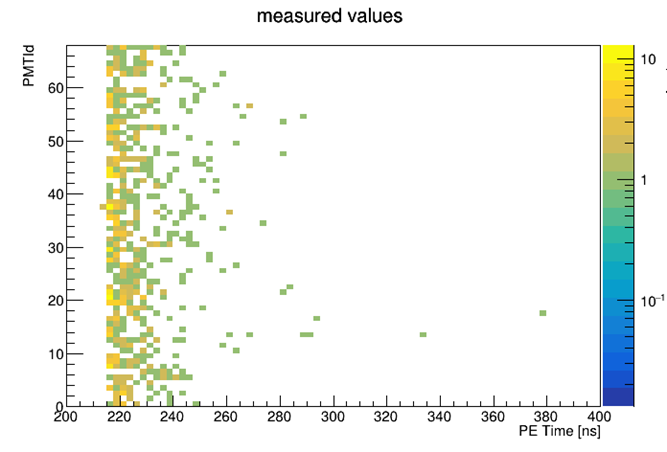
\includegraphics[width=0.45\linewidth]{figures/selections/DSNB-observed.png}
    }
    \subfigure[expected PE number]{
        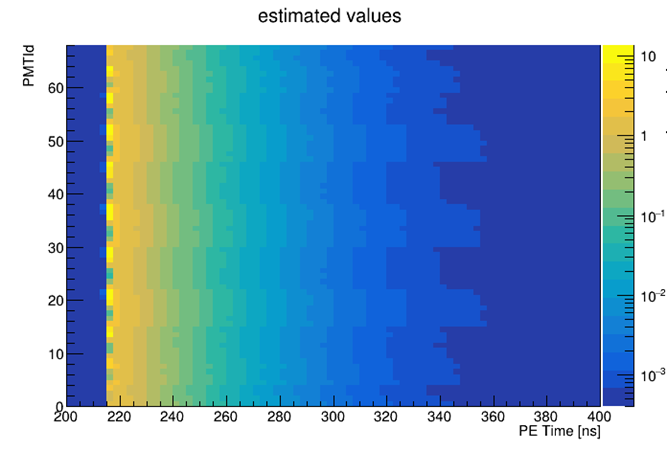
\includegraphics[width=0.45\linewidth]{figures/selections/DSNB-expected.png}
    }
    \caption{The observed and expected PE number distribution in a DSNB prompt event.}
    \label{fig:dist-goodness}
\end{figure}

The goodness $\chi^2$ is then calculated with $n, \nu$:

\begin{equation}
    \chi_P^2 = 2 \sum_{i=1}^N \left( n_i \log \frac{n_i}{\nu_i} + \nu_i - n_i \right)
    \label{equ:chi2}
\end{equation}

Only when $n_i \neq 0$, the NDF is counted, and the $\chi_P^2$ is accumulated.

With (\ref{equ:chi2}), the fitting goodness of each prompt event is obtained. For DSNB prompt events and atomspheric-neutrino prompt events, $\chi_P^2-E_k$ distributions are plotted and compared, as shown in figure \ref{fig:sel-goodness}. We remove events with prompt $(\chi_P^2, E_k)$ outside the red-line parallelogram.

\begin{figure}[!htb]
    \centering
    \subfigure[DSNB]{
        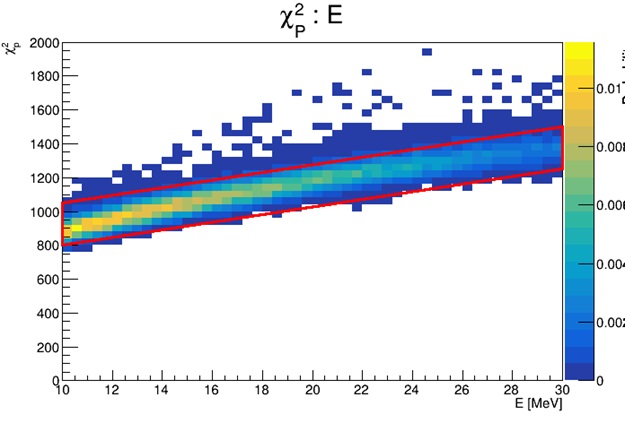
\includegraphics[width=0.45\linewidth]{figures/sensitivity/sel-goodness-srn.png}
    }
    \subfigure[atmos]{
        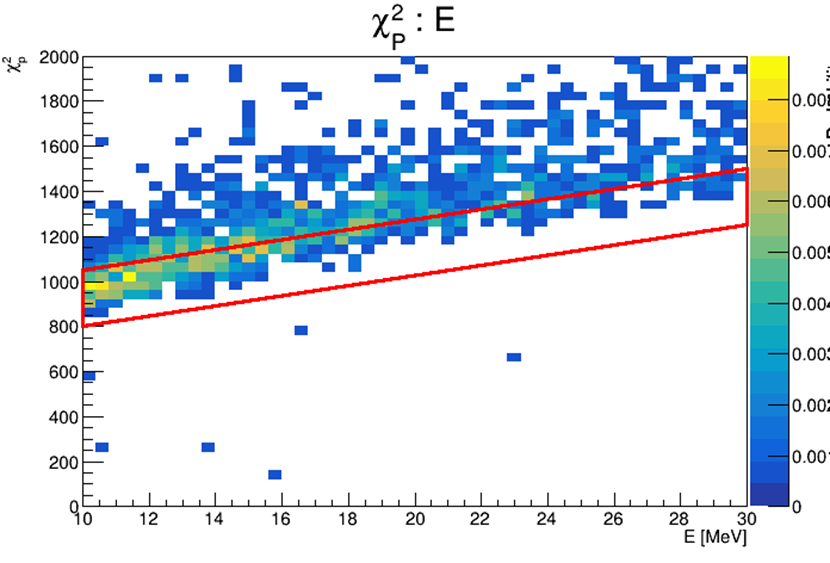
\includegraphics[width=0.45\linewidth]{figures/sensitivity/sel-goodness-o16nue-.png}
    }
    \caption{The joint distribution of goodness and energy. The red lines show the region retained.}
    \label{fig:sel-goodness}
\end{figure}

拟合优度 $\chi_P^2$ 的计算：

\begin{equation}
    \chi_P^2 = 2 \sum_{i=1}^N \left( n_i \log \frac{n_i}{\nu_i} + \nu_i - n_i \right)
\end{equation}

根据 \cite{cowan_statistical_1998}，当 $n_i = 0$ 时，$n_i \log \frac{n_i}{\nu_i} = 0$，仍需计算 $\nu_i - n_i$，并加入到 $\chi_P^2$ 中

自由度: $\mathrm{NDF} = N - m - 1$，其中 $N = 80 \times 68 = 5440$ 为总计格点个数， $m = 7$ 为重建的参数个数，包括能量、位置（3）、时间、方向（2）7维信息。故：

下面展示了几个 goodness 的计算方法
\begin{enumerate}
    \item （错误）计算 PE 时空分布的期望值 $\nu_{ij}$ ，统计测量值 $n_{ij}$，按 (\ref{equ:chi2}) 计算 $\chi^2_P$。分 bin $80 \times 68$，$80$ 表示 $t^{res} \in [200, 400] \si{\nano\second}$，每 bin 宽度 $\SI{2.5}{\nano\second}$。$68$ 表示 6444 支 PMT，分入 68 区间。计算 $\chi^2_P$ 时 $n_{ij}=0$ 的 bin 不计入计算。
      
    \item 计算 PE 时空分布的期望值 $\nu_{ij}$ ，统计测量值 $n_{ij}$，按 (\ref{equ:chi2}) 计算 $\chi^2_P$。分 bin $80 \times 68$，$80$ 表示 $t^{res} \in [200, 400] \si{\nano\second}$，每 bin 宽度 $\SI{2.5}{\nano\second}$。$68$ 表示 6444 支 PMT，分入 68 区间。$\mathrm{NDF} = 80 \times 68 - 7 - 1 = 5432$
    
    \item 计算 PE 时空分布的期望值 $\nu_{ij}$ ，统计测量值 $n_{ij}$，按 (\ref{equ:chi2}) 计算 $\chi^2_P$。分 bin $200 \times 6444$，$200$ 表示 $t^{res} \in [200, 400] \si{\nano\second}$，每 bin 宽度 $\SI{1}{\nano\second}$。$6444$ 表示 6444 支 PMT。 $\mathrm{NDF} = 200 \times 6444 - 7 - 1 = 1288792$

    \item 直接代入拟合结果，计算似然函数的负对数，$- \ln{f(n_i^{obs}, t_{ij} | \vec{\theta})}$，似然函数如式 (\ref{equ:likelihood})
\end{enumerate}

\begin{figure}[!htb]
    \centering
    \subfigure[DSNB $\chi_P^2$]{
        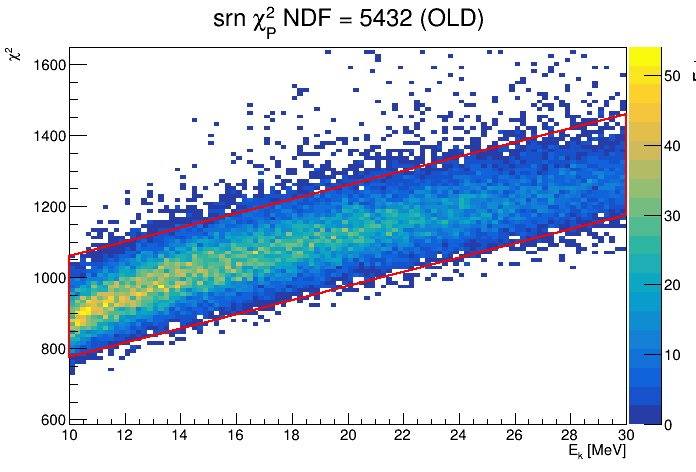
\includegraphics[width=0.45\linewidth]{figures/selections/goodness/srn-80-68-old.png}
    }
    \subfigure[大气中微子 $\chi_P^2$]{
        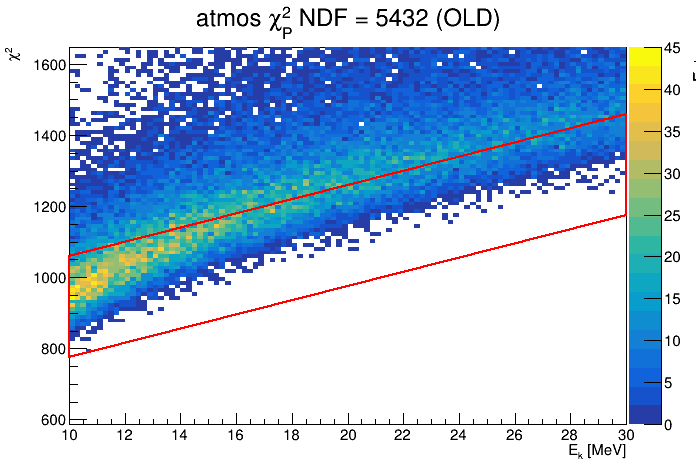
\includegraphics[width=0.45\linewidth]{figures/selections/goodness/atmos-80-68-old.png} 
    }
    \caption{$\mathrm{NDF} = 5432$ (错误的计数方法)}
\end{figure}
\begin{figure}[!htb]
    \centering
    \subfigure[DSNB $\chi_P^2$]{
        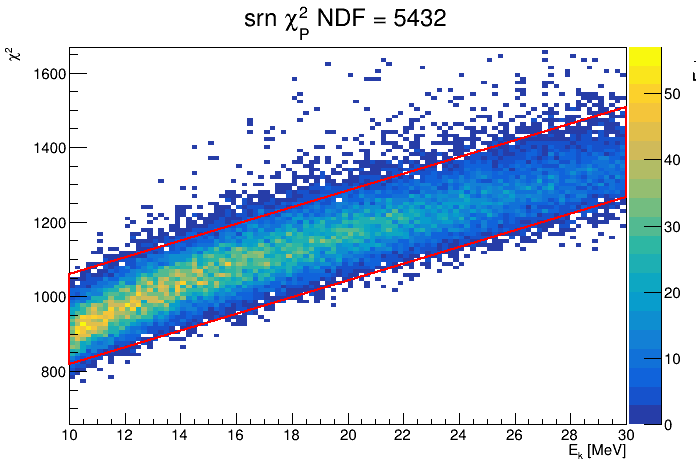
\includegraphics[width=0.45\linewidth]{figures/selections/goodness/srn-80-68.png}
    }
    \subfigure[大气中微子 $\chi_P^2$]{
        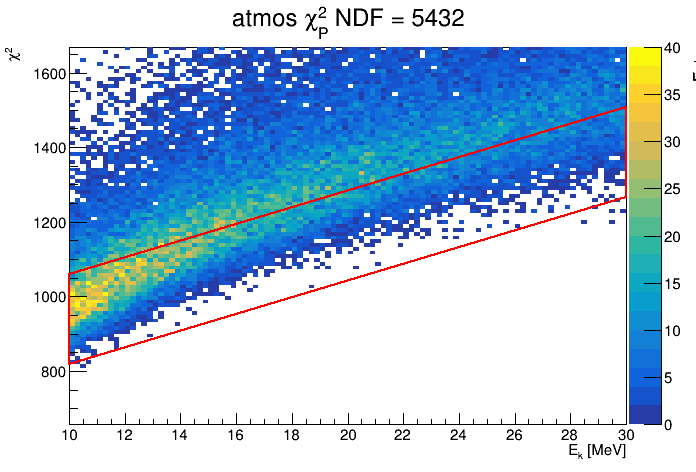
\includegraphics[width=0.45\linewidth]{figures/selections/goodness/atmos-80-68.png} 
    }
    \caption{$\mathrm{NDF} = 5432$}
\end{figure}
 \begin{figure}[!htb]
    \centering
    \subfigure[DSNB $\chi_P^2$]{
        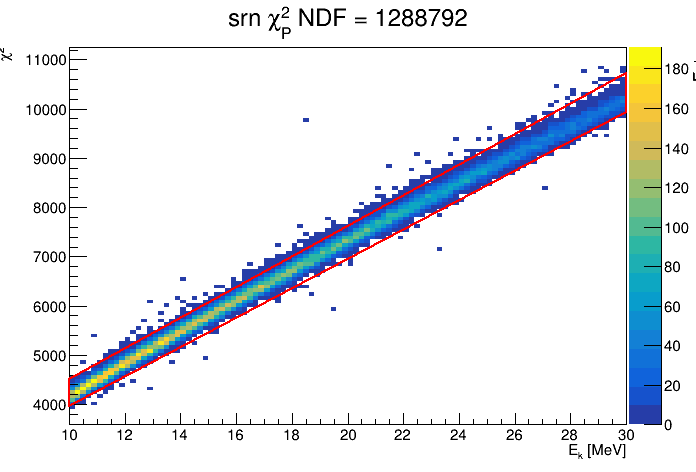
\includegraphics[width=0.45\linewidth]{figures/selections/goodness/srn-200-6444.png}
    }
    \subfigure[大气中微子 $\chi_P^2$]{
        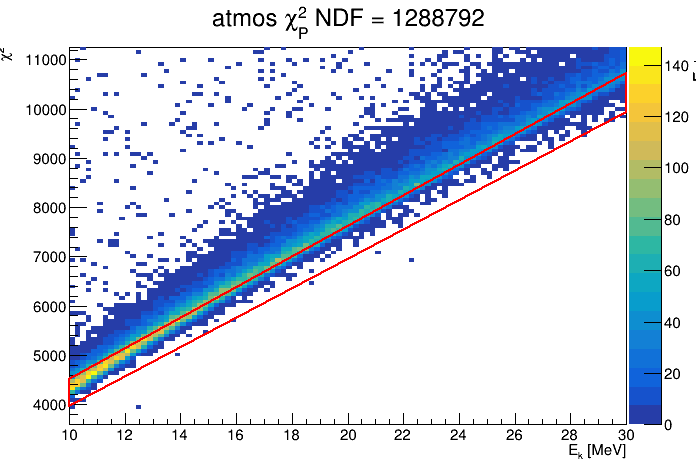
\includegraphics[width=0.45\linewidth]{figures/selections/goodness/atmos-200-6444.png} 
    }
    \caption{$\mathrm{NDF} = 1288792$}
\end{figure}
\begin{figure}[!htb]
    \centering
    \subfigure[DSNB $\chi_P^2$]{
        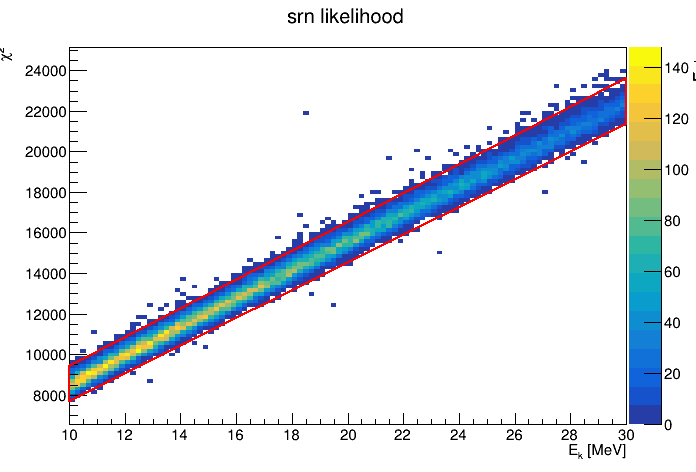
\includegraphics[width=0.45\linewidth]{figures/selections/goodness/srn-likelihood.png}
    }
    \subfigure[大气中微子 $\chi_P^2$]{
        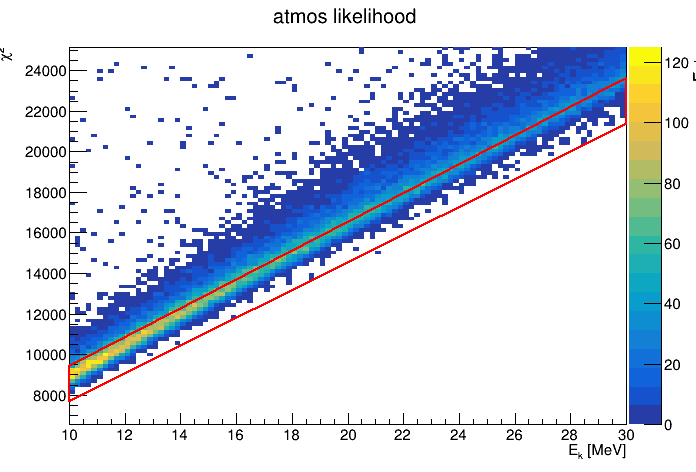
\includegraphics[width=0.45\linewidth]{figures/selections/goodness/atmos-likelihood.png} 
    }
    \caption{似然函数的负对数}
\end{figure}

% \begin{figure}[!htb]
%     \centering
%     \subfigure[抛弃0的 80*68 bins: 不抛弃 0 的 80*68 bins]{
%         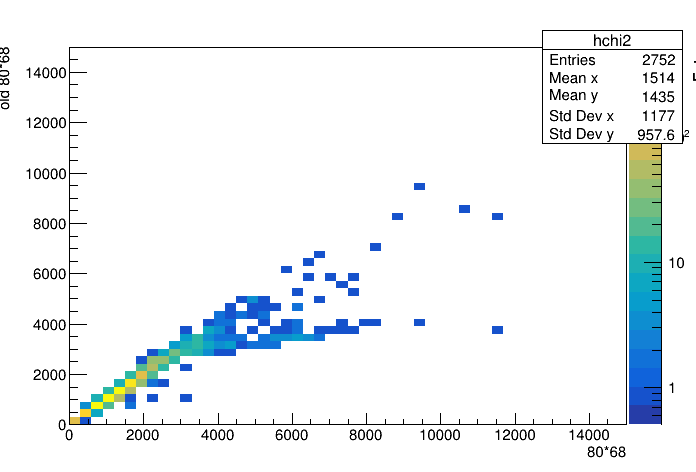
\includegraphics[width=0.45\linewidth]{figures/selections/goodness/neo-80-68.png}
%     }
%     \subfigure[200*6444 bins: 80*68 bins]{
%         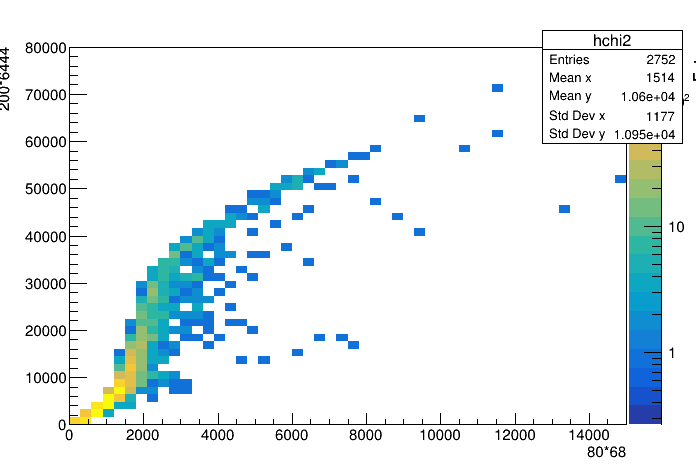
\includegraphics[width=0.45\linewidth]{figures/selections/goodness/neo-200-6444.png} 
%     }
%     \caption{三种卡方计算方法对比：抛弃 0 的 80*68 bins、不抛弃 0 的 80*68 bins、不抛弃 0 的 200*6444 bins}
% \end{figure}

现在计算不同方法的选择效率 $\epsilon$，表示为：
\begin{equation}
    \epsilon_{goodness} = \frac{N_{goodness}}{N_{previos}}
\end{equation}

其中 $N_{previos}$ 表示通过之前的判选之后剩余的事例数（之前的判选包括快慢信号符合、快信号能量判选）；$N_{goodness}$ 表示通过之前的判选之后，进一步通过拟合优度判选的事例数。

并计算相对信噪比
\begin{equation}
    \frac{\epsilon_{DSNB}}{\epsilon_{Atmos}}
\end{equation}

\begin{table}[!htb]
    \centering
    \caption{不同方法计算的拟合优度判选，其选择效率}
    \begin{tabular}{cccc}
        \hline
        拟合优度方法 & DSNB & 大气中微子 & 相对信噪比 \\
        \hline
        \makecell{$\chi_P^2 (Wrong)$ \\ $\mathrm{NDF} = 5432$} & $96.1\%$ & $37.9\%$ & $2.54$ \\
        \hline
        \makecell{$\chi_P^2$ \\ $\mathrm{NDF} = 5432$} & $95.4\%$ & $35.1\%$ & $2.72$ \\
        \hline
        \makecell{$\chi_P^2$ \\ $\mathrm{NDF} = 1288792$} & $98.8\%$ & $32.1\%$ & $3.07$ \\
        \hline
        $-\ln{f(n_i^{obs}, t_{ij} | \vec{\theta})}$ & $99.1\%$ & $47.3\%$ & $2.09$ \\
        \hline
    \end{tabular}
\end{table}

故采用 $\chi_P^2 (\mathrm{NDF} = 200 \times 6444 - 7 - 1 = 1288792)$，作为拟合优度指标，信噪比相比此前的错误算法，提升约 $21\%$
\subsection{Cherenkov-ring compliance}

\begin{figure}[!htb]
    \centering
    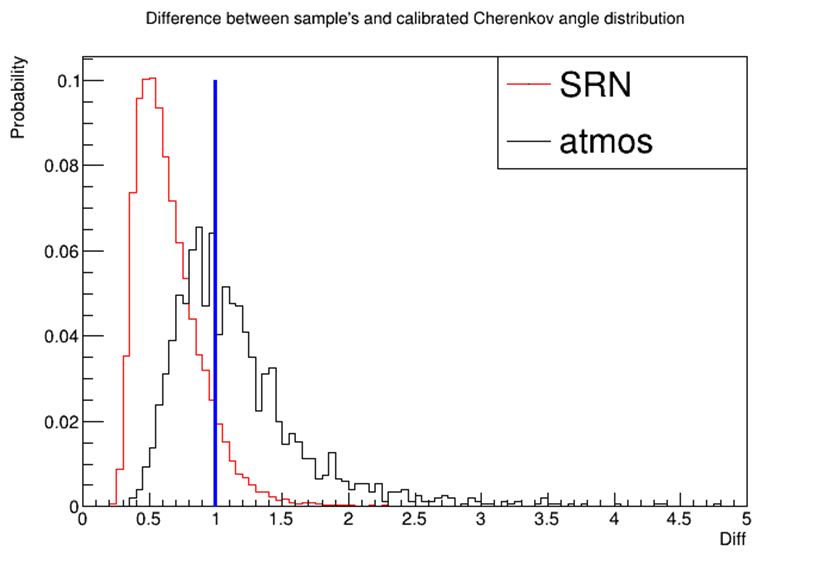
\includegraphics[width=0.5\linewidth]{figures/sensitivity/sel-cherenkov-ring.png}
    \caption{The compliance shows how a hit pattern is similar to a cherenkov ring. The less value, the closer pattern.}
    \label{fig:sel-ring}
\end{figure}

\paragraph{事例展示}

为了直观展示不同 PMT 的位置关系和事例的切伦科夫环，将球面上的点 $(\theta, \phi)$ 投影到平面坐标 $(\tilde{\theta}, \tilde{\phi})$。本投影中的 $\theta$ 是 PMT 位置的球面极角，与下文用于判选的 PE 相对重建事例方向的夹角不同。投影如下：
\begin{equation}
    \begin{aligned}
        & \tilde{\theta} = \frac{1.3}{\sqrt{1 + \sin \theta \cdot \sin \phi / 2}} \cos \theta \\
        & \tilde{\phi} = \frac{-2}{\sqrt{1 + \sin \theta \cdot \sin \phi / 2}} \sin \theta \cdot \cos \frac{\phi}{2}
    \end{aligned}
\end{equation}

对于球面上的 6444 支 PMT，我们展示每一支原来的 $(\theta, \phi)$，以及它们投影之后的参数 $(\tilde{\theta}, \tilde{\phi})$

\begin{figure}[!htb]
    \centering
    \subfigure[$\theta: (\tilde{\theta}, \tilde{\phi})$]{
        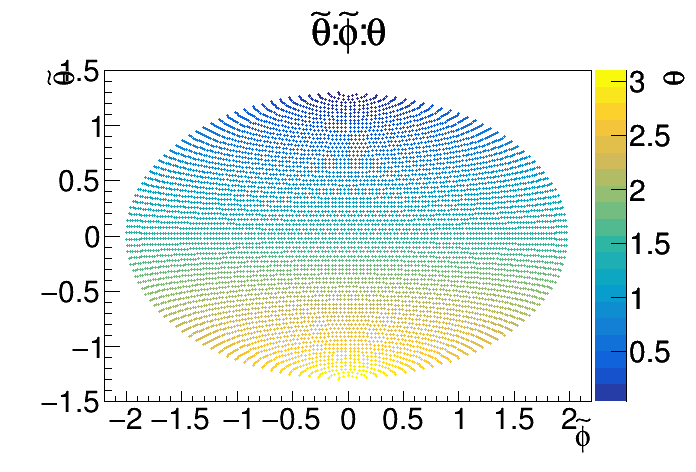
\includegraphics[width=0.45\linewidth]{figures/selections/thetac/xytheta.png}
    }
    \subfigure[$\phi: (\tilde{\theta}, \tilde{\phi})$]{
        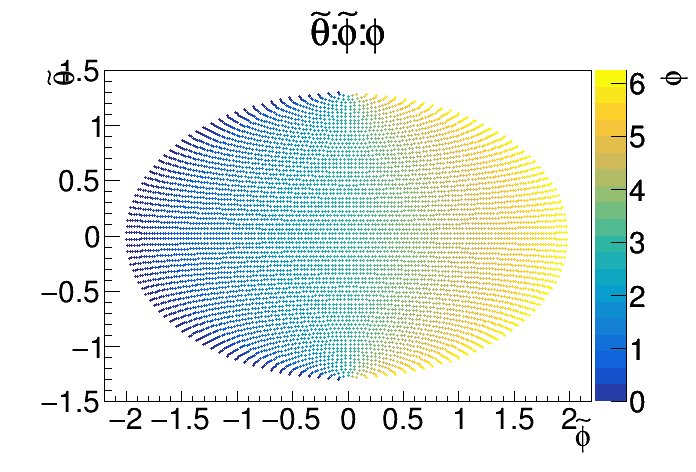
\includegraphics[width=0.45\linewidth]{figures/selections/thetac/xyphi.png}
    }
    \caption{6444 支 PMT 的投影}
\end{figure}

判选思路：

\begin{itemize}
    \item 对于 DSNB 信号，快信号为正电子，其切伦科夫角分布通常接近正电子模板，在 $\cos\theta \approx 0.7$ 附近具有明显峰值。
    \item 部分大气中微子本底包含多个方向不同的次级带电粒子，例如多个 $\gamma$ 产生的电子，或 $\mu^\pm$ 及伴随的强子活动，其切伦科夫角分布更分散，与正电子模板的偏离较大。产生正电子快信号的本底仍可能通过此判选。
\end{itemize}

根据两者切伦科夫光角分布的形状差异进行判选，以一维 $\cos\theta$ 分布作为环形态的指标。

当前方法并不通过固定时间残差窗口对 PE 做硬分类，而是使用每个 PE 的切伦科夫后验概率作为权重。切伦科夫成分同时包含直入射和非直入射成分；一个 PE 可以按概率分配到切伦科夫光和闪烁光两类，例如贡献 $0.9$ CPE 和 $0.1$ SPE。

图 \ref{fig:chev-pattern} 保留了基于时间残差的旧版快信号展示，用于直观说明环结构，不作为当前后验概率加权判选的结果图。

\begin{figure}[!htb]
    \centering
    \subfigure[DSNB]{
        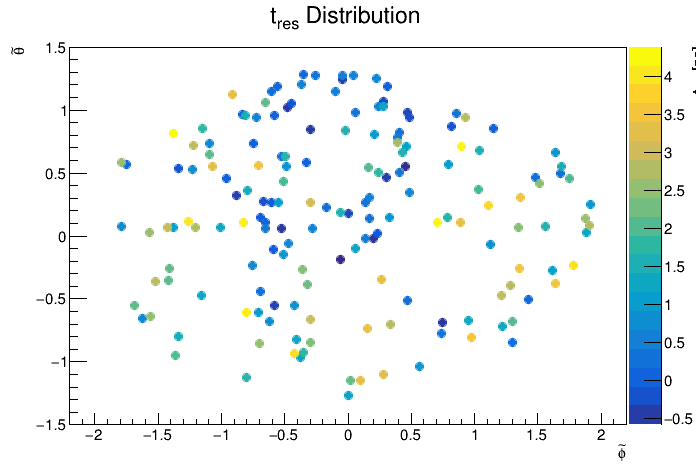
\includegraphics[width=0.45\linewidth]{figures/selections/thetac/srn-15-dist.png}
    }
    \subfigure[大气中微子]{
        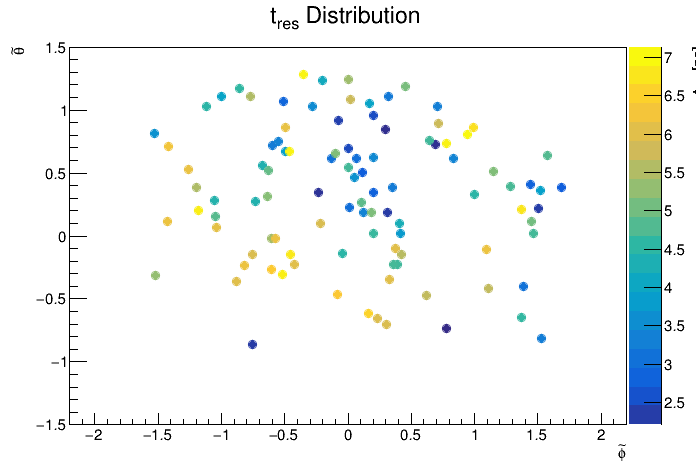
\includegraphics[width=0.45\linewidth]{figures/selections/thetac/atmos-9115-dist.png} 
    }
    \caption{DSNB 和大气中微子事例的旧版快信号环结构示意，颜色表示时间残差。当前判选采用切伦科夫后验概率加权，而非本图的时间残差展示方式。}
    \label{fig:chev-pattern}
\end{figure}

对于快信号中的每个 PE，使用重建顶点 $\boldsymbol{x}_{\mathrm{reco}}$、重建事例单位方向 $\hat{\boldsymbol{d}}_{\mathrm{reco}}$ 和命中 PMT 的位置 $\boldsymbol{r}_{\mathrm{PMT},j}$，定义夹角 $\theta_j$：
\begin{equation}
    \cos\theta_j = \hat{\boldsymbol{d}}_{\mathrm{reco}} \cdot
    \frac{\boldsymbol{r}_{\mathrm{PMT},j}-\boldsymbol{x}_{\mathrm{reco}}}
    {|\boldsymbol{r}_{\mathrm{PMT},j}-\boldsymbol{x}_{\mathrm{reco}}|}.
\end{equation}

以 PE 的切伦科夫后验概率 $w_j^C$ 为权重填充 $\cos\theta$ 直方图，并归一化得到各 bin 的观测概率 $n_i$：
\begin{equation}
    n_i = \frac{\sum_{j\in i} w_j^C}{\sum_j w_j^C}, \qquad \sum_i n_i = 1.
\end{equation}

通过正电子模拟标定归一化的 $\cos\theta$ 预期分布 $\nu_i$，满足 $\sum_i\nu_i=1$。

图 \ref{fig:chev-cos} 展示了当前方法得到的两个单事例角分布 $n_i$，和预期分布 $\nu_i$ 的对比，明显可以看到，DSNB 事例比大气中微子事例更契合预期分布。

\begin{figure}[!htb]
    \centering
    \subfigure[DSNB]{
        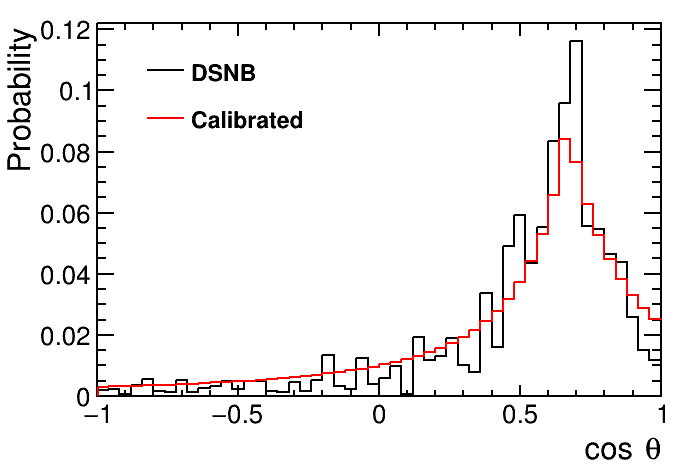
\includegraphics[width=0.45\linewidth]{figures/selections/thetac/srn-30-2.png}
    }
    \subfigure[大气中微子]{
        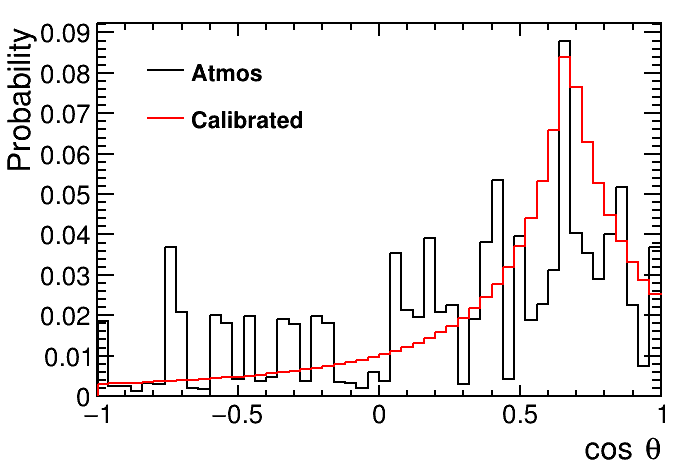
\includegraphics[width=0.45\linewidth]{figures/selections/thetac/atmos-61-2.png}
    }
    \caption{按切伦科夫后验概率加权并归一化的快信号 $\cos\theta$ 分布：DSNB 事例（左）和大气中微子事例（右），红线表示由正电子模拟标定的固定 $\cos\theta$ 模板 $\nu_i$。纵轴为各 bin 的概率。}
    \label{fig:chev-cos}
\end{figure}

采用与拟合优度 cut 相同形式的统计量比较预期分布 $\nu_i$ 与观测分布 $n_i$。拟合优度比较二维直方图，这里比较一维归一化角分布：

\begin{equation}
    \chi_{\mathrm{chev}}^2 = 2\sum_i\left(n_i\ln\frac{n_i}{\nu_i}+\nu_i-n_i\right).
\end{equation}

由于两个分布均归一化到 1，此统计量衡量角分布形状与正电子模板的偏离，而不直接比较切伦科夫 PE 总量。$\chi_{\mathrm{chev}}^2$ 越小，角分布越接近正电子模板。对于 $n_i=0$ 的 bin，取 $n_i\ln(n_i/\nu_i)=0$。

图 \ref{fig:chev-selection} 展示了信号与本底的 $\chi_{\mathrm{chev}}^2$ 随快信号重建能量的分布，以及当前采用的判选边界。

\begin{figure}[!htb]
    \centering
    \subfigure[DSNB]{
        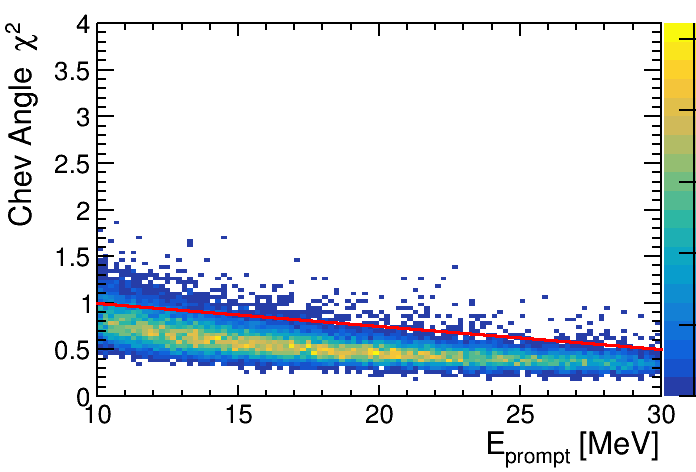
\includegraphics[width=0.45\linewidth]{figures/selections/thetac/latest-indep-srn-chevangle-e.png}
    }
    \subfigure[大气中微子]{
        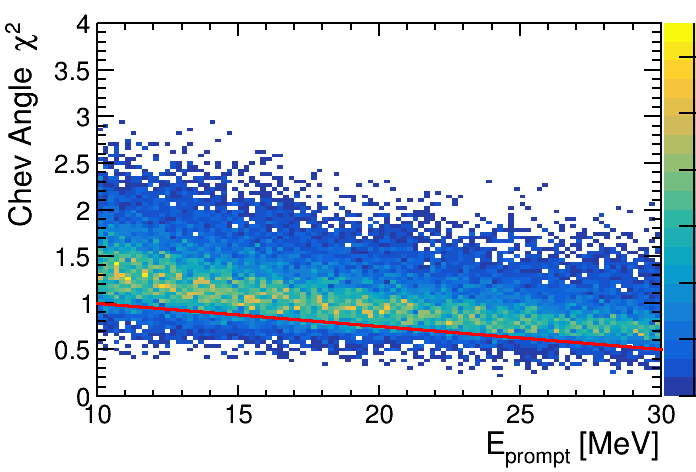
\includegraphics[width=0.45\linewidth]{figures/selections/thetac/latest-indep-all-chevangle-e.png}
    }
    \caption{独立考察角分布判选时，DSNB（左）和大气中微子（右）的 $\chi_{\mathrm{chev}}^2$--$E_{\mathrm{prompt}}$ 分布。红线为当前随能量变化的判选边界，保留红线下方的事例。}
    \label{fig:chev-selection}
\end{figure}

保留满足下式的事例作为后续判选的候选：
\begin{equation}
    \chi_{\mathrm{chev}}^2 < -0.025\,\frac{E_{\mathrm{prompt}}}{\si{\MeV}}+1.25.
\end{equation}
该边界根据模拟中 DSNB 信号与大气中微子本底的分布目测选定，目标是尽量保留 DSNB 事例并减少保留的大气中微子事例，目前尚未进行定量的参数扫描优化。

当前方法的局限与后续优化方向：

\begin{itemize}
    \item 当前使用固定正电子模板，尚未考虑角分布对能量和顶点位置的依赖。
    \item 当前判选边界由目测确定，后续可通过参数扫描定量优化，并评估信号效率与本底保留率的权衡。
\end{itemize}
\subsection{cherenkov photon emitting ability}

\begin{figure}[!htb]
    \centering
    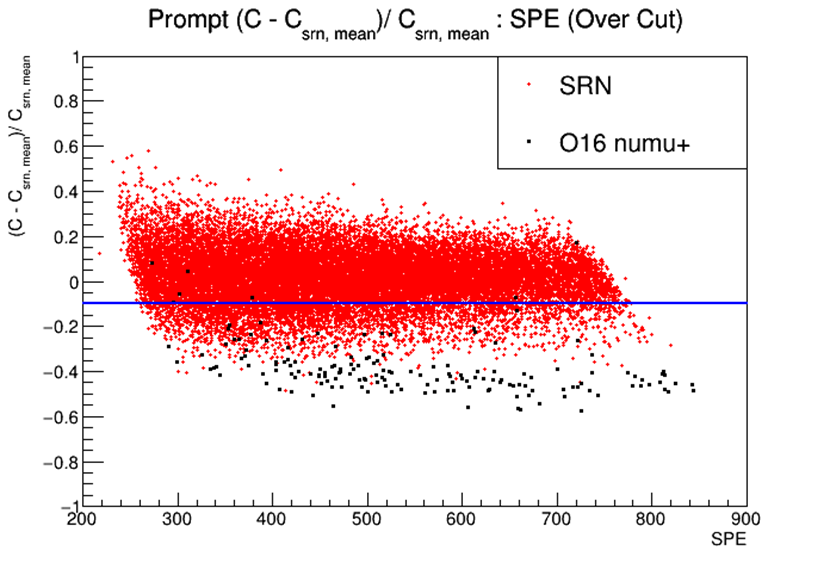
\includegraphics[width=0.5\linewidth]{figures/sensitivity/sel-csr.png}
    \caption{The Cherenkov photon number compared with scintillation one. The more an event is like an electron event, the bigger the relative Cherenkov photon number is.}
    \label{fig:sel-csr}
\end{figure}

\subsection{selection efficiency}

\begin{table}[!htb]
    \caption{Event rates after selections}
    \begin{tabular}{rrrrr}
        \hline
         & DSNB & Atmos NC & Atmos $\bar{\nu}_e$ CC & Atmos $\bar{\nu}_{\mu} / \nu_{\mu}$ CC \\
        \hline
        Before cut & & & & \\
        Coincidence & & & & \\
        Goodness & & & & \\
        Cut-2 & & & & \\
        Cut-3 & & & & \\
        \hline
    \end{tabular}
\end{table}

After all the cuts are applied, the DSNB even rate remains $1.68 (\SI{20}{\kilo\tonne year})^{-1}$, the atmospheric neutrino event rate decreases to $0.0212 (\SI{20}{\kilo\tonne year})^{-1}$

\subsection{判选条件重复问题}
\subsubsection{要讨论的两个判选条件}

\begin{table}[!htb]
    \centering
    \caption{要讨论的两个判选条件}
    \begin{tabular}{ccc}
        \hline
        编号 & 名称 & 判选表达式 \\
        \hline
        cut-1 & 拟合优度 & $\chi_P^2 < 310 * \frac{E_{prompt}}{\si{\MeV}} + 1412$ \\
        cut-3 & 切伦科夫光发光能力 & $\frac{CPE - (0.3 * SPE - 8)}{0.3 * SPE - 8} > -0.1$ \\
        \hline
    \end{tabular}
\end{table}

\subsubsection{问题描述}

我们基于电子模型重建事例顶点 $(E, t_0, \vec{x}, \vec{d})$，也基于电子模型重建 SPE、CPE \ref{equ:nc-recon}。

假设有一我们不知道粒子类型的事例，只要这个事例的重建较好，我们就可以认为这个事例是类似电子的。因此这个事例的切伦科夫光、闪烁光的比例也应该和电子接近

那么切伦科夫光发光能力的判选，是否和拟合优度的判选重复？

\subsubsection{讨论}

我们将两个判选条件做线性变换，重写为：

\begin{equation}
    \begin{aligned}
        I_{\chi_P^2} & = -\chi_P^2 + 310 * \frac{E_{prompt}}{\si{\MeV}} + 1412 & > 0 \\
        I_{chev} & = \frac{CPE - (0.3 * SPE - 8)}{0.3 * SPE - 8} + 0.1 & > 0
    \end{aligned}
\end{equation}

$I_{\chi_P^2}$ 表示拟合的好坏，数值越大，拟合结果越好，事例越像电子

$I_{chev}$ 表示事例中切伦科夫光的相对闪烁光有多少，数值越大，切伦科夫光越多

下面我们将展示这两个指标的二维分布

\begin{figure}[!htb]
    \centering
    \subfigure[DSNB]{
        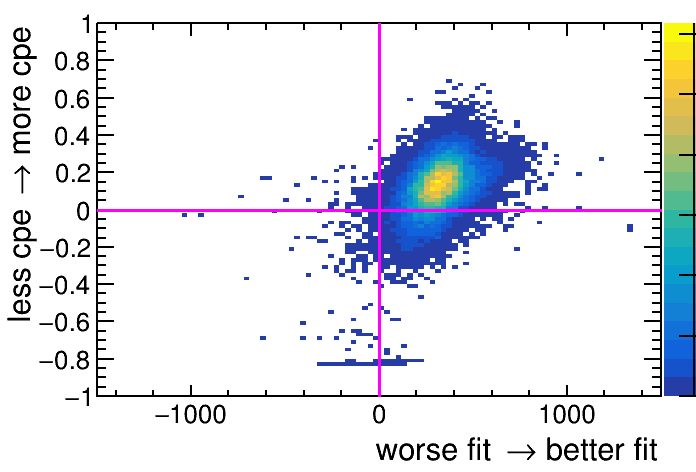
\includegraphics[width=0.45\linewidth]{figures/selections/indicator-srn-old.png}
    }
    \subfigure[大气中微子]{
        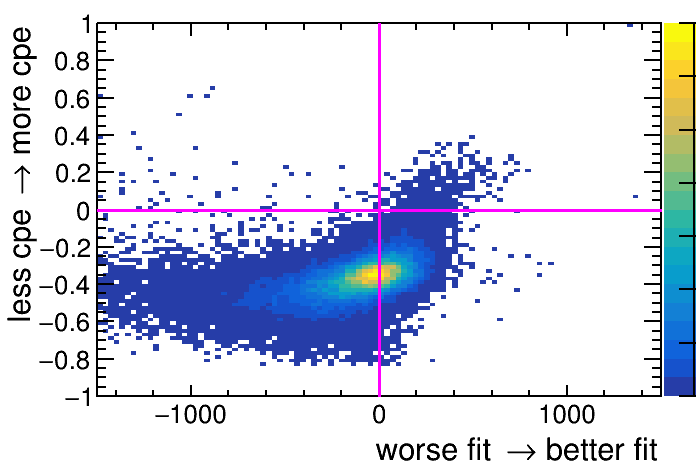
\includegraphics[width=0.45\linewidth]{figures/selections/indicator-atmos-old.png} 
    }
    \caption{横轴表示拟合好坏，横轴表示切伦科夫光相对多少，粉线标注判选条件，第一象限为通过}
\end{figure}

可以看到，和我们想的一样，拟合好的事例切伦科夫光都比较多，拟合差的事例切伦科夫光都比较少

\paragraph{为什么之前觉得切伦科夫光判选能额外筛掉事例}

之前的拟合优度判选条件（cut-1）设置得比较松，切伦科夫光判选条件（cut-3）设置得比较严格。

之前出现 cut-1 留下的大气中微子事例，被 cut-3 筛掉。我们认为这些事例，是拟合比较好，但是切伦科夫光较少。而实际情况是之前 cut-1 比较松，这些事例拟合得也没有那么好。

\paragraph{改进}

把 cut-1 也设置更严格一些，例如要求 $I_{\chi_P^2} > 200$，如图：

\begin{figure}[!htb]
    \centering
    \subfigure[DSNB]{
        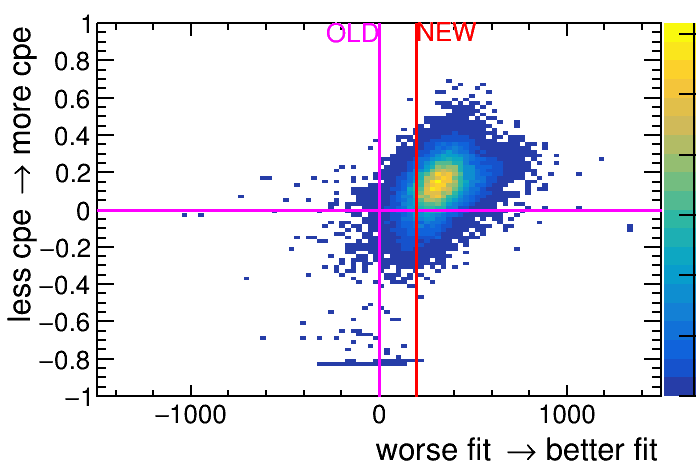
\includegraphics[width=0.45\linewidth]{figures/selections/indicator-srn.png}
    }
    \subfigure[大气中微子]{
        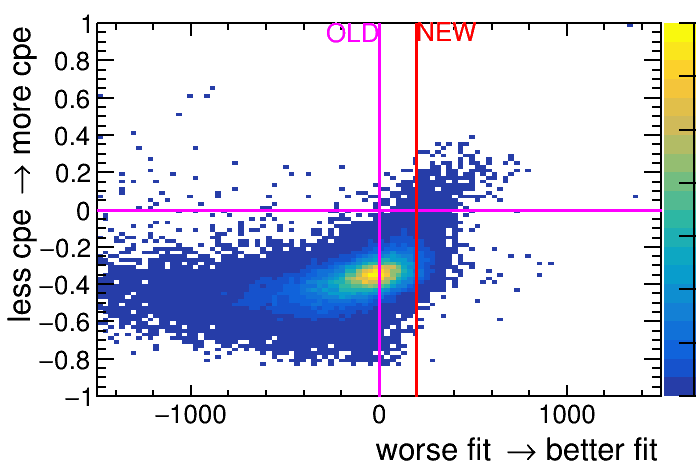
\includegraphics[width=0.45\linewidth]{figures/selections/indicator-atmos.png} 
    }
    \caption{横轴表示拟合好坏，横轴表示切伦科夫光相对多少，粉线和红线标注判选条件，第一象限为通过}
\end{figure}

这样两个判选条件看起来一样严格了。我们验证一下选择效率：

\begin{table}[!htb]
    \centering
    \caption{两种判选条件的选择效率和相关系数}
    \begin{tabular}{ccccc}
        \hline
        & cut-1 效率 & cut-3 效率 & 联合效率 & 相关系数 \\
        \hline
        DSNB & 85.5 \% & 84.5 \% & 75.9 \% & 0.29 \\
        大气中微子 & 4.7 \% & 1.1 \% & 0.6 \% &  0.27 \\
        % 相对信噪比 & 18.2 & 76.8 & 127 & \\
        \hline
    \end{tabular}
\end{table}

其中相关系数为：

\begin{equation}
    \rho = \frac{\varepsilon_{13}  - \varepsilon_1 \varepsilon_3}{\sqrt{\varepsilon_1 (1 - \varepsilon_1) \varepsilon_3 (1 - \varepsilon_3)}}
\end{equation}

附上原来的选择效率：

\begin{table}[!htb]
    \centering
    \caption{两种判选条件的选择效率和相关系数（旧）}
    \begin{tabular}{ccccc}
        \hline
        & cut-1 效率 & cut-3 效率 & 联合效率 & 相关系数 \\
        \hline
        DSNB & 99.1 \% & 84.5 \% & 84.2 \% & 0.15\\
        大气中微子 & 32.2 \% & 1.1 \% & 0.8 \% & 0.10 \\
        % 信噪比 & 3.1 & 76.8 & 105 & \\
        \hline
    \end{tabular}
\end{table}

\newpage
\section{Selection Results and Residual Backgrounds}
\subsection{Event classification and selection metrics}
\begin{table}[!htb]
    \centering
    \caption{判选条件和需要事例指标}
    \begin{tabular}{c|cccc}
        \hline
        & 简称 & 判选条件 & 展示指标 \\
        \hline
        cut-0 & 快慢信号符合 & \makecell{$t \le \SI{20}{\micro\second}$ \\ $E_{prompt} \in [10, 30]$ \\ $E_{delayed}$} & $E_{prompt}$, $E_{delayed}$ \\
        cut-1 & 拟合优度 & $\chi_{fit}^2 < 331 \times E_{prompt} + 1212$ & $-\chi_{fit}^2 + 331 \times E_{prompt} + 1212$ \\
        cut-2 & 切伦科夫光角分布 & $\chi_{chev}^2 < - \frac{1}{40} E_{prompt} + 1.25$ & $-\chi_{chev}^2 - \frac{1}{40} E_{prompt} + 1.25$ \\
        cut-3 & C/S 比例 & $\frac{CPE}{0.3 \times SPE - 8} > 1$ & $\frac{CPE}{0.3 \times SPE - 8} - 1$ \\
        \hline
    \end{tabular}
\end{table}

\subsection{Event rates through successive selections}

我们对大气中微子事例依次应用以上判选条件。下图中，我们展示按第一层级分类的不同大气中微子事例的各指标。这些指标展示每类事例在各个 cut 下的表现，如图 \ref{fig:layer1-cut1}，展示的是各类事例的拟合优度好坏，指标越大，事例拟合得越好，而我们只保留 $x>0$ 事例作为信号候选。可以从图中看到，大部分大气中微子事例的拟合都是不够好的。

\begin{figure}[!htb]
    \centering
    \subfigure[快信号能量]{
        \includegraphics[width=0.45\linewidth]{../../dsnb/types-progress/layer1/prompt.png}
    }
    \subfigure[慢信号能量]{
        \includegraphics[width=0.45\linewidth]{../../dsnb/types-progress/layer1/delayed.png} 
    }
    \subfigure[cut-1 指标]{
        \includegraphics[width=0.45\linewidth]{../../dsnb/types-progress/layer1/good.png}
        \label{fig:layer1-cut1}
    }
    \subfigure[cut-2 指标]{
        \includegraphics[width=0.45\linewidth]{../../dsnb/types-progress/layer1/thetac.png} 
    }
    \subfigure[cut-3 指标]{
        \includegraphics[width=0.45\linewidth]{../../dsnb/types-progress/layer1/csr.png} 
    }
    \caption{按中微子味道和反应道分类的不同中微子事例的各指标}
\end{figure}

可以看到，经过所有判选之后，在 \SI{22.5}{\kilo\tonne year} 的曝光量下，大气中微子事例剩余 $5 \times 10^{-3}$，主要来自 $\bar{\nu}_{\mu}$ $NC$ ($2 \times 10^{-3}$) 以及 $\bar{\nu}_e$ $CC$ ($2 \times 10^{-3}$)。

容易猜到，$\bar{\nu}_e$ $CC$ 反应道中大量无法被判选条件排除的事例是 $\bar{\nu}_e + \ce{^{1}H} \to e^+ + n$，这些事例和信号基本相同，因此难以被判选条件区分出来。所以，接下来我们可以查看 $\bar{\nu}_{\mu}$ $NC$ 事例的第二层级分类，即按反应的核素分类。下图中，我们展示这些事例的各个指标。

\begin{figure}[!htb]
    \centering
    \subfigure[快信号能量]{
        \includegraphics[width=0.45\linewidth]{../../dsnb/types-progress/layer2-iso/nc-numu-/prompt.png}
    }
    \subfigure[慢信号能量]{
        \includegraphics[width=0.45\linewidth]{../../dsnb/types-progress/layer2-iso/nc-numu-/delayed.png} 
    }
    \subfigure[cut-1 指标]{
        \includegraphics[width=0.45\linewidth]{../../dsnb/types-progress/layer2-iso/nc-numu-/good.png}
        \label{fig:layer2-cut1}
    }
    \subfigure[cut-2 指标]{
        \includegraphics[width=0.45\linewidth]{../../dsnb/types-progress/layer2-iso/nc-numu-/thetac.png} 
    }
    \subfigure[cut-3 指标]{
        \includegraphics[width=0.45\linewidth]{../../dsnb/types-progress/layer2-iso/nc-numu-/csr.png} 
    }
    \caption{按不同核素分类的 $\bar{\nu}_{\mu}$ $NC$ 大气中微子事例的各指标}
\end{figure}

可以看到过阈事例主要来自 $\bar{\nu}_{\mu} + \ce{^{16}O}$ 与 $\bar{\nu}_{\mu} + \ce{^{35}Cl}$。我们可以继续深入，研究 $\bar{\nu}_{\mu}$ 在这两种核素下产生的大气中微子事例末态，究其根源找到是什么事例通过我们的三轮判选。

\begin{figure}[!htb]
    \centering
    \subfigure[快信号能量]{
        \includegraphics[width=0.45\linewidth]{../../dsnb/types-progress/layer3-iso/nc-O16numu-/prompt.png}
    }
    \subfigure[慢信号能量]{
        \includegraphics[width=0.45\linewidth]{../../dsnb/types-progress/layer3-iso/nc-O16numu-/delayed.png} 
    }
    \subfigure[cut-1 指标]{
        \includegraphics[width=0.45\linewidth]{../../dsnb/types-progress/layer3-iso/nc-O16numu-/good.png}
        \label{fig:layer3-O16-cut1}
    }
    \subfigure[cut-2 指标]{
        \includegraphics[width=0.45\linewidth]{../../dsnb/types-progress/layer3-iso/nc-O16numu-/thetac.png} 
    }
    \subfigure[cut-3 指标]{
        \includegraphics[width=0.45\linewidth]{../../dsnb/types-progress/layer3-iso/nc-O16numu-/csr.png} 
    }
    \caption{按末态粒子分类的 $\bar{\nu}_{\mu} + \ce{^{16}O}$ $NC$ 大气中微子事例的各指标}
\end{figure}

\begin{figure}[!htb]
    \centering
    \subfigure[快信号能量]{
        \includegraphics[width=0.45\linewidth]{../../dsnb/types-progress/layer3-iso/nc-Cl35numu-/prompt.png}
    }
    \subfigure[慢信号能量]{
        \includegraphics[width=0.45\linewidth]{../../dsnb/types-progress/layer3-iso/nc-Cl35numu-/delayed.png} 
    }
    \subfigure[cut-1 指标]{
        \includegraphics[width=0.45\linewidth]{../../dsnb/types-progress/layer3-iso/nc-Cl35numu-/good.png}
        \label{fig:layer3-Cl35-cut1}
    }
    \subfigure[cut-2 指标]{
        \includegraphics[width=0.45\linewidth]{../../dsnb/types-progress/layer3-iso/nc-Cl35numu-/thetac.png} 
    }
    \subfigure[cut-3 指标]{
        \includegraphics[width=0.45\linewidth]{../../dsnb/types-progress/layer3-iso/nc-Cl35numu-/csr.png} 
    }
    \caption{按末态粒子分类的 $\bar{\nu}_{\mu} + \ce{^{35}Cl}$ $NC$ 大气中微子事例的各指标}
\end{figure}

最后我们发现，留下来的是事例率为 $2 \times 10^{-4}$ 的 $\bar{\nu}_{\mu} + \ce{^{16}O} \to \bar{\nu}_{\mu} + \ce{^{15}O} + n$ 事例，以及事例率为 $9 \times 10^{-5}$ 的 $\bar{\nu}_{\mu} + \ce{^{35}Cl} \to \bar{\nu}_{\mu} + \ce{^{34}Cl} + n$ 事例。根据误差棒我们可以推断，这两类事例，最后过阈的都各只有一个，下表将展示这两个事例的情况。

\begin{table}[!htb]
    \centering
    \caption{两个 $\bar{\nu}_{\mu} + \ce{^{A}N} \to \bar{\nu}_{\mu} + \ce{^{A-1}N} + n$ 事例}
    \begin{tabular}{ccc}
        \hline
        & \ce{^{16}O} & \ce{^{35}Cl}  \\
        \hline
        入射 $\bar{\nu}_{\mu}$ 动能 [MeV] & 250.87 & \\
        末态 $\bar{\nu}_{\mu}$ 动能 [MeV] & 189.39 & \\
        中子动能 [MeV] & 28.37 & \\
        \hline
        快信号能量 [MeV] & 14.55 & 11.86 \\
        慢信号能量 [MeV] & 0.39 & 0.46 \\
        \hline
        $\chi_{fit}^2$ & 5671 & 4871 \\
        指标 1 & 65 & 28 \\
        \hline
        $\chi_{chev}^2$ & 0.74 & 0.74 \\
        指标 2 & 0.15 & 0.15 \\
        \hline
        快信号 CPE & 98 & 79 \\
        快信号 SPE & 367 & 308 \\
        指标 3 & 0.05 & 0.04 \\
        \hline
    \end{tabular}
\end{table}

$\bar{\nu}_{\mu} + \ce{^{16}O} \to \bar{\nu}_{\mu} + \ce{^{15}O} + n$ 事例中的中子，在其产生的第 $\SI{6.14}{\nano\second}$，与探测器中的 \ce{^{16}O} 反应：$n + \ce{^{16}O} \to \ce{^{16}O} + n + 3 \gamma$，其中 $3 \gamma$ 的动能总和为 $\SI{11.08}{\MeV}$，与 DSNB 信号的正电子快信号行为相似，导致该事例通过判选。
\subsection{Selection efficiencies across flavour, isotope, and final state}
上一小节我们展示了大气中微子过阈的绝对事例率，本小节将展示各类大气中微子事例的选择效率，从而横向对比三轮判选不同核素、不同中微子味道、不同末态的不同效果。

定义 $\eta_1$ 为事例过 cut-1 的效率，$\eta_{12}$ 为事例同时过 cut-1/2 的效率，$\eta_{123}$ 为事例同时过 cut-1/2/3 所有判选的效率，下面我们将从不同侧面展示这三个效率

首先，假设固定大气中微子味道为 $\bar{\nu}_{\mu}$，我们可以对比不同末态事例的选择效率，也可以对比不同核素产生的中微子事例的选择效率，如图 \ref{fig:eff-numubar}

\begin{figure}[!htb]
    \centering
    \subfigure[不同核素事例的选择效率 $\eta_{1}$]{
        \includegraphics[width=0.3\linewidth]{../../dsnb/efficiency/flavour/numu-/curst-e1.png}
    }
    \subfigure[不同核素事例的选择效率 $\eta_{12}$]{
        \includegraphics[width=0.3\linewidth]{../../dsnb/efficiency/flavour/numu-/curst-e12.png}
    }
    \subfigure[不同核素事例的选择效率 $\eta_{123}$]{
        \includegraphics[width=0.3\linewidth]{../../dsnb/efficiency/flavour/numu-/curst-e123.png}
    }
    \subfigure[不同末态事例的选择效率 $\eta_{1}$]{
        \includegraphics[width=0.3\linewidth]{../../dsnb/efficiency/flavour/numu-/isotope-e1.png}
    }
    \subfigure[不同末态事例的选择效率 $\eta_{12}$]{
        \includegraphics[width=0.3\linewidth]{../../dsnb/efficiency/flavour/numu-/isotope-e12.png}
    }
    \subfigure[不同末态事例的选择效率 $\eta_{123}$]{
        \includegraphics[width=0.3\linewidth]{../../dsnb/efficiency/flavour/numu-/isotope-e123.png}
    }
    \caption{$\bar{\nu}_{\mu}$ 大气中微子事例选择效率}
    \label{fig:eff-numubar}
\end{figure}

同样地，如果固定核素为 \ce{^{16}O}, 我们可以对比不同中微子味道的事例，或不同末态的事例，如图 \ref{fig:eff-O16}

\begin{figure}[!htb]
    \centering
    \subfigure[不同味道事例的选择效率 $\eta_{1}$]{
        \includegraphics[width=0.3\linewidth]{../../dsnb/efficiency/isotope/O16/curst-e1.png}
    }
    \subfigure[不同味道事例的选择效率 $\eta_{12}$]{
        \includegraphics[width=0.3\linewidth]{../../dsnb/efficiency/isotope/O16/curst-e12.png}
    }
    \subfigure[不同味道事例的选择效率 $\eta_{123}$]{
        \includegraphics[width=0.3\linewidth]{../../dsnb/efficiency/isotope/O16/curst-e123.png}
    }
    \subfigure[不同末态事例的选择效率 $\eta_{1}$]{
        \includegraphics[width=0.3\linewidth]{../../dsnb/efficiency/isotope/O16/flavour-e1.png}
    }
    \subfigure[不同末态事例的选择效率 $\eta_{12}$]{
        \includegraphics[width=0.3\linewidth]{../../dsnb/efficiency/isotope/O16/flavour-e12.png}
    }
    \subfigure[不同末态事例的选择效率 $\eta_{123}$]{
        \includegraphics[width=0.3\linewidth]{../../dsnb/efficiency/isotope/O16/flavour-e123.png}
    }
    \caption{\ce{^{16}O} 大气中微子事例选择效率}
    \label{fig:eff-O16}
\end{figure}

最后，如果固定末态为 $\nu + N + n$，即一个中子的 NC 末态，我们可以对比不同中微子味道的事例，或不同核素的事例，如图 \ref{fig:eff-nu-n}

\begin{figure}[!htb]
    \centering
    \subfigure[不同味道事例的选择效率 $\eta_{1}$]{
        \includegraphics[width=0.3\linewidth]{../../dsnb/efficiency/curst/nu_n/flavour-e1.png}
    }
    \subfigure[不同味道事例的选择效率 $\eta_{12}$]{
        \includegraphics[width=0.3\linewidth]{../../dsnb/efficiency/curst/nu_n/flavour-e12.png}
    }
    \subfigure[不同味道事例的选择效率 $\eta_{123}$]{
        \includegraphics[width=0.3\linewidth]{../../dsnb/efficiency/curst/nu_n/flavour-e123.png}
    }
    \subfigure[不同核素事例的选择效率 $\eta_{1}$]{
        \includegraphics[width=0.3\linewidth]{../../dsnb/efficiency/curst/nu_n/isotope-e1.png}
    }
    \subfigure[不同核素事例的选择效率 $\eta_{12}$]{
        \includegraphics[width=0.3\linewidth]{../../dsnb/efficiency/curst/nu_n/isotope-e12.png}
    }
    \subfigure[不同核素事例的选择效率 $\eta_{123}$]{
        \includegraphics[width=0.3\linewidth]{../../dsnb/efficiency/curst/nu_n/isotope-e123.png}
    }
    \caption{含一个中子的 NC 末态事例选择效率}
    \label{fig:eff-nu-n}
\end{figure}

\newpage
\section{Sensitivity Study}
\[P_s = \sum_{i=a}^b \mathrm{Poisson(i, \mu_{bkg})}\]

where $b$ is the nearest integer around $S + \mu_{bkg}$, and $a$ is determined by $b$, both of which are on the same horizontal level in the probability distribution.
\[\mathrm{Poisson} (a, \mu_{bkg}) \ge \mathrm{Poisson} (b, \mu_{bkg}) \]
\[\mathrm{Poisson} (a - 1, \mu_{bkg}) \le \mathrm{Poisson} (b, \mu_{bkg}) \]

\begin{figure}[!htb]
    \centering
    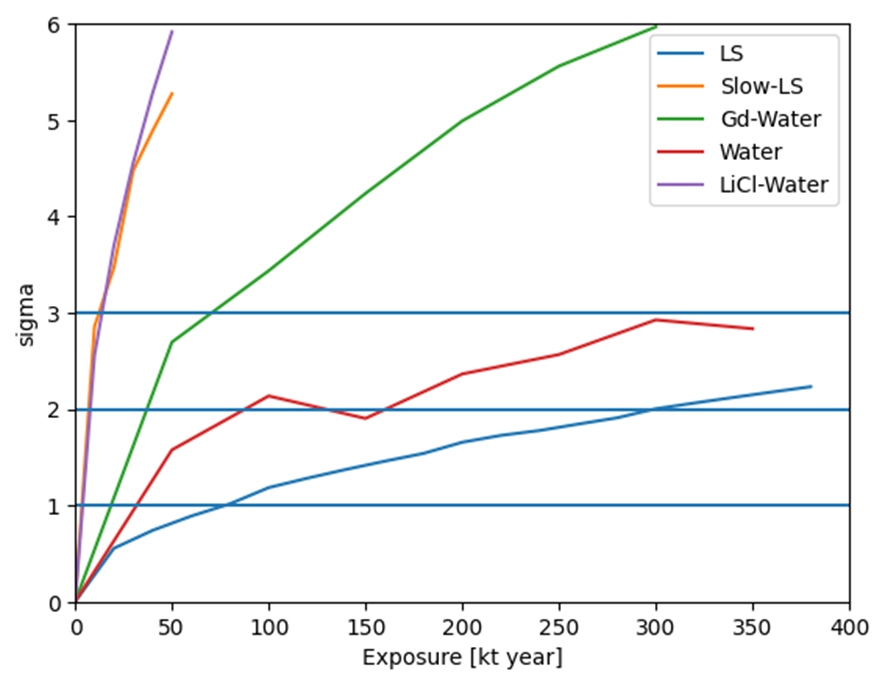
\includegraphics[width=0.5\linewidth]{figures/sensitivity/sensitivity.png}
    \caption{DSNB detection sensitivity with different types of detectors}
    % Discovery potential for supernova relic neutrinos with slow liquid scintillator detectors
    \label{fig:sensitivity}
\end{figure}

It can be found that in the LiCl water solution detector, the sensitivity of DSNB is the greatest, slightly greater than that in the Slow-LS detector.

\newpage
\section{Summary}

\newpage
\section{Appendix: 讨论遇到的问题}
\subsection{拟合优度算法比较及个例研究}
\textbf{好像这些图没办法看出差别，暂时没意义，或者想一想更好的表现形式}

取一个 DNSB 事例，$\chi_P^2 = 5600 @ \SI{14.46}{\MeV}$，另取一个大气中微子事例（$\ce{{}^{16}O} + \bar{\nu}_e$，NC 反应道，末态为多个中子）$\chi_P^2 = 12254 @ \SI{14.95}{\MeV}$，对比两者逐 bin 的 $\chi_P^2$

\begin{figure}[!htb]
    \centering
    \subfigure[DSNB $\chi_P^2 = 5600 @ \SI{14.46}{\MeV}$]{
        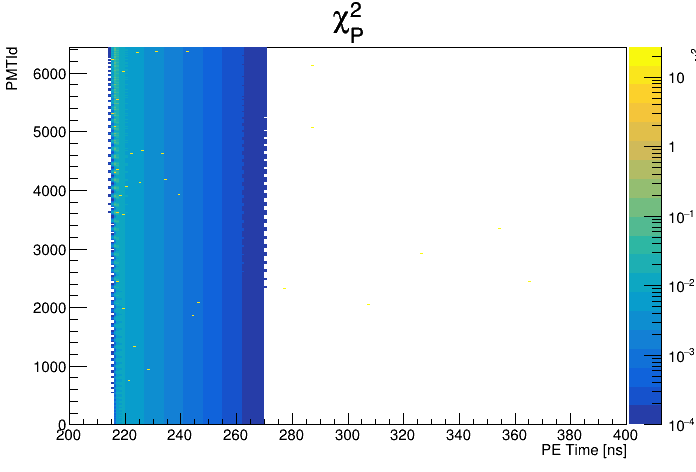
\includegraphics[width=0.45\linewidth]{figures/selections/goodness/srn-chi2.png}
    }
    \subfigure[大气中微子 $\chi_P^2 = 12254 @ \SI{14.95}{\MeV}$]{
        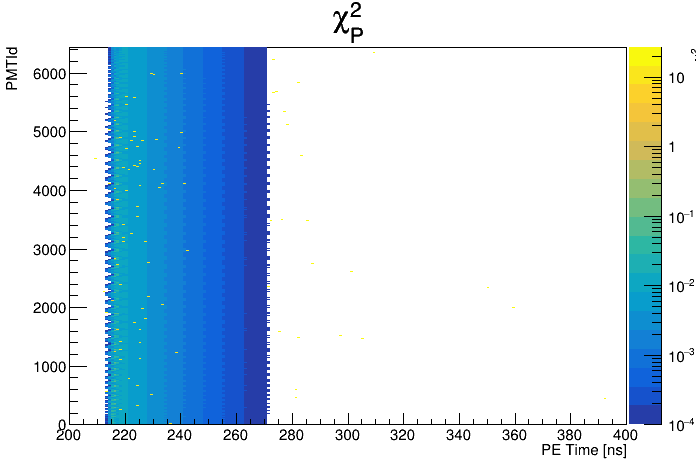
\includegraphics[width=0.45\linewidth]{figures/selections/goodness/atmos-chi2.png} 
    }
    \caption{一个 DSNB 和大气中微子快信号逐 bin $\chi_P^2$ 对比}
\end{figure}

\begin{figure}[!htb]
    \centering
    \subfigure[预期]{
        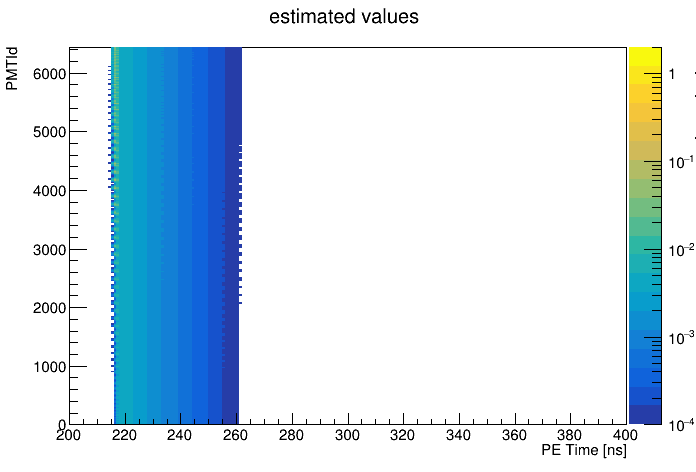
\includegraphics[width=0.45\linewidth]{figures/selections/goodness/srn-v.png}
    }
    \subfigure[实测]{
        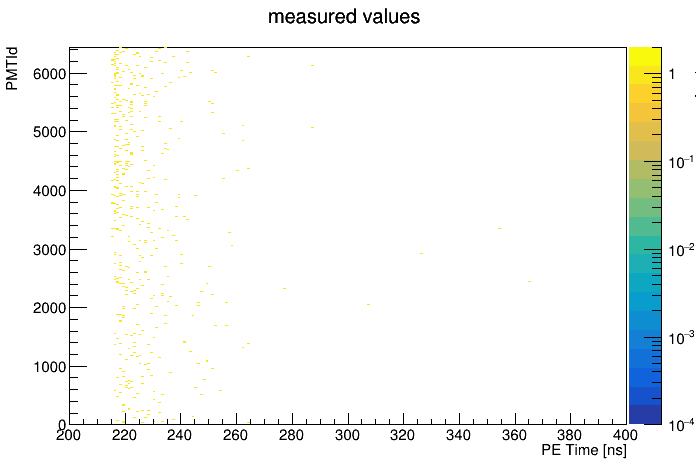
\includegraphics[width=0.45\linewidth]{figures/selections/goodness/srn-n.png} 
    }
    \caption{DSNB $\chi_P^2 = 5600 @ \SI{14.46}{\MeV}$}
\end{figure}

\begin{figure}[!htb]
    \centering
    \subfigure[预期]{
        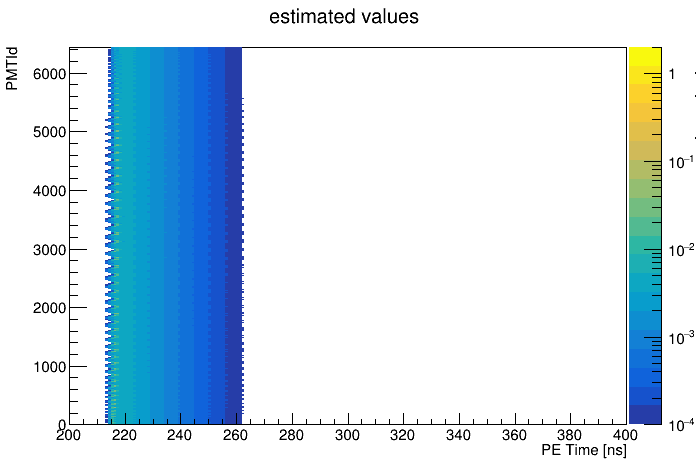
\includegraphics[width=0.45\linewidth]{figures/selections/goodness/atmos-v.png}
    }
    \subfigure[实测]{
        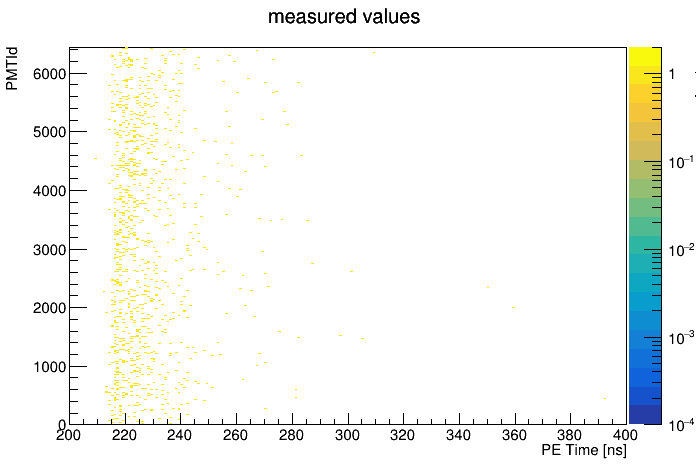
\includegraphics[width=0.45\linewidth]{figures/selections/goodness/atmos-n.png} 
    }
    \caption{大气中微子 $\chi_P^2 = 12254 @ \SI{14.95}{\MeV}$}
\end{figure}

\subsection{大气中微子末态分类选择效率}
\textbf{待整理}
\subsection{方法局限和待完善内容}
\textbf{待完善：} NC 末态和 CC 末态可以分在两个图里

\subsection{待做}

\begin{itemize}
    \item \textbf{在大气中微子分类整理的部分开头，核心问题是信号特征，信号是什么特征，为什么需要为末态分类}
    \item \textbf{把所有味道中微子的 NC、CC 末态表格都搬到文章里。图片需要放大}
    \item \textbf{重做所有图片，放大图片里面的文字}
\end{itemize}

\bibliographystyle{IEEEtran}
\bibliography{reference}

\end{document}
